\documentclass{book}
% comment out the following line if you want to latex the whole book:
%\includeonly{ch9}
  % preamble

\usepackage{verbatim}\usepackage{epsf}
\usepackage{framed}
\usepackage{html}
\usepackage[dvipdfm]{graphicx}
\usepackage[thmmarks,standard,framed,thref]{ntheorem}

%
% The complete documentation of this ntheorem package is in
% ntheorem.ps
% 
\theoremstyle{break}
\newtheorem{Exercise}{Exercise}[chapter]
\newframedtheorem{Code}{Code}[chapter]
\newframedtheorem{Output}{Output}[chapter]
%\newtheorem{Code}{Code}[chapter]
%\newtheorem{Output}{Output}[chapter]

%
% If you want to add new box, just add a line like
%
%\newframedtheorem{foo}{foo}[chapter]
%
% this will make the foo environment, numbered sequentially within
% chapter, available. So if you say
%
% \begin{foo}
% This is first sample of foo.
% \end{foo}
% You will see this in a framed box
%
% To get a list of this foo box, you need to say something like
%
%\chapter*{List of foos}
%\addcontentsline{toc}{chapter}{List of foos}
%\theoremlisttype{allname}
%\listtheorems{foo}
%
% first two lines are just to make this list looks like list of
% figures and list of tables. 

\setlength{\textwidth}{ 5.45in}           % default seems to be around 4.8 inch,
\addtolength{\evensidemargin}{-0.4in}  % so we can devide the extra 0.65 inch
\addtolength{\oddsidemargin}{-0.4in}   % over left and right margin

\setlength{\parindent}{2.5em}
\setlength{\parskip}{1.2 ex plus0.2ex minus 0.1ex}
\renewcommand{\baselinestretch}{1.05}
\renewcommand{\floatpagefraction}{1.0}
\renewcommand{\topfraction}{1.0}

\begin{htmlonly}
\setlength{\textheight}{30in}
\end{htmlonly}

\begin{document}
  \frontmatter
\makebox[3.5in][s]{}\verb=Time-stamp: <2002-04-12 13:22:51 piet>=
%
% nice latex feature: you can specify which files you want to include in your
% next output, by listing only those files as arguments to \includeonly{} 
% above on the third line (I had to put this comment here, since the emacs
% time stamp is only recognized in the first eight lines).
% NOTE: if you want to print out the whole book, simply comment out the line
% starting with \includeonly above.
%
% It is a good idea to write this top level file out, each time a change has
% been made, in order to get the correct time stamp to appear on the title
% page.  Even if you print out only one chapter, still the title page will
% appear, so that the time stamp will be include (otherwise the time stamp
% would appear uselessly on a separate white page, before the chapter).
%
    \def\simlt{\hbox{ \rlap{\raise 0.425ex\hbox{$<$}}\lower 0.65ex\hbox{$\sim$} }}
\def\simgt{\hbox{ \rlap{\raise 0.425ex\hbox{$>$}}\lower 0.65ex\hbox{$\sim$} }}
\def\({\left(}
\def\){\left)}
\def\[{\left[}
\def\]{\left]}
\def\half{{\ifmmode{{1 \over 2}}\else{${1 \over 2}$}\fi}}
\def\dhalf{{\textstyle {1 \over 2}}}
\def\threehalf{{\ifmmode{{3 \over 2}}\else{${3 \over 2}$}\fi}}
\def\dthreehalf{{\textstyle {3 \over 2}}}
\def\dfivehalf{{\textstyle {5 \over 2}}}
\def\dfivethree{{\textstyle {5 \over 3}}}
\def\hhalf{{\textstyle\frac{1}{2}}}
\def\quarter{{\textstyle\frac{1}{4}}}
\def\one#1{{\textstyle\frac{1}{#1}}}
\def\three#1{{\textstyle\frac{3}{#1}}}
\def\seven#1{{\textstyle\frac{7}{#1}}}
\def\E{{\cal E}}
\def\bx{{\bf x}}
\def\br{{\bf r}}
\def\bv{{\bf v}}
\def\ba{{\bf a}}
\def\bb{{\bf b}}
\def\bj{{\bf j}}
\def\bs{{\bf s}}
\def\bc{{\bf c}}
\def\bp{{\bf p}}
\def\bk{{\bf k}}
\def\badot{{\bf \dot a}}
\def\batwo{{{\bf  a}^{(2)}}}
\def\bathree{{{\bf  a}^{(3)}}}
\def\bR{{\bf R}}
\def\bV{{\bf V}}
           % input, not include, since all files need the \def{}
    % title page

\thispagestyle{empty}                 % suppresses page numbering of first page

\begin{latexonly}

\begin{center}


\hbox{}

\bigskip\bigskip


{\lggggb Moving Stars Around}

\bigskip


\bigskip\bigskip


{\lggb A Preliminary Version}


\medskip


{\lggb of what will expand into}


\medskip

{\lggb Volumes 1,2,3}

\medskip

{\lggb of the series}

\bigskip\bigskip

{\lgggb The Art of Computational Science}

\bigskip\bigskip

\end{center}

\end{latexonly}


\begin{htmlonly}


\begin{center}


\hbox{}

\bigskip\bigskip


{\huge \bf Moving Stars Around}

\medskip


{\LARGE A Preliminary Version}



{\LARGE of what will expand into}


\medskip



{\LARGE Volumes 1,2,3}

\medskip



{\LARGE of the series}


\bigskip


{\huge \bf The Art of Computational Science}



\bigskip


\end{center}
\end{htmlonly}

 \begin{latexonly}
 \begin{center}
 \leavevmode
 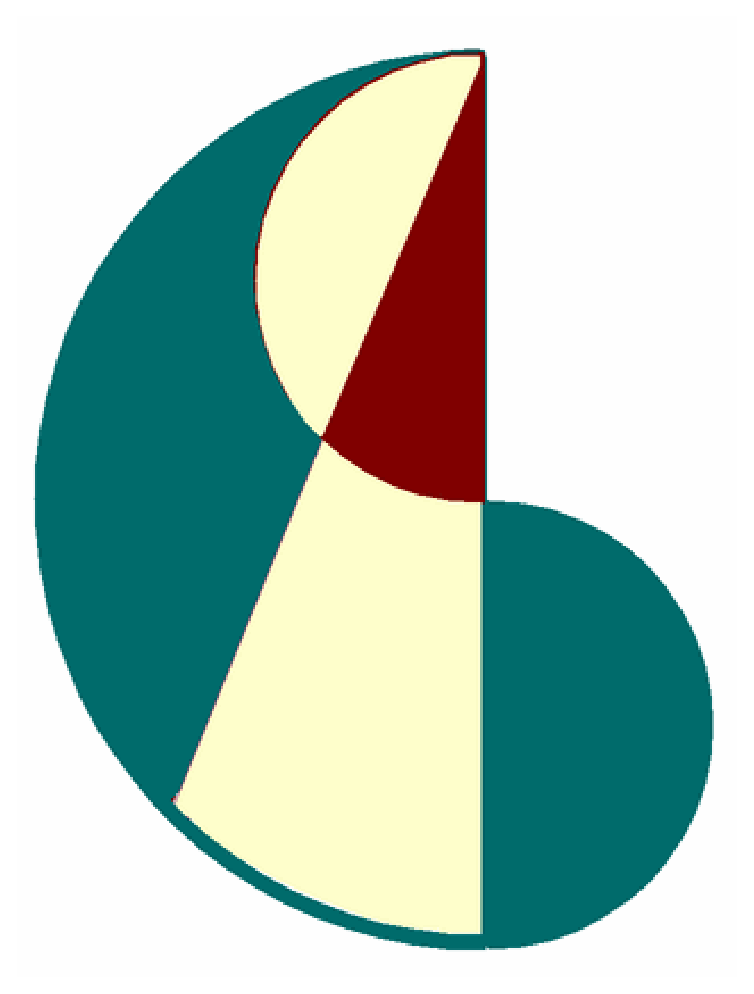
\includegraphics[width=4cm]{acstitle.eps}
 \end{center}
 \end{latexonly}


\begin{htmlonly}
\begin{center}
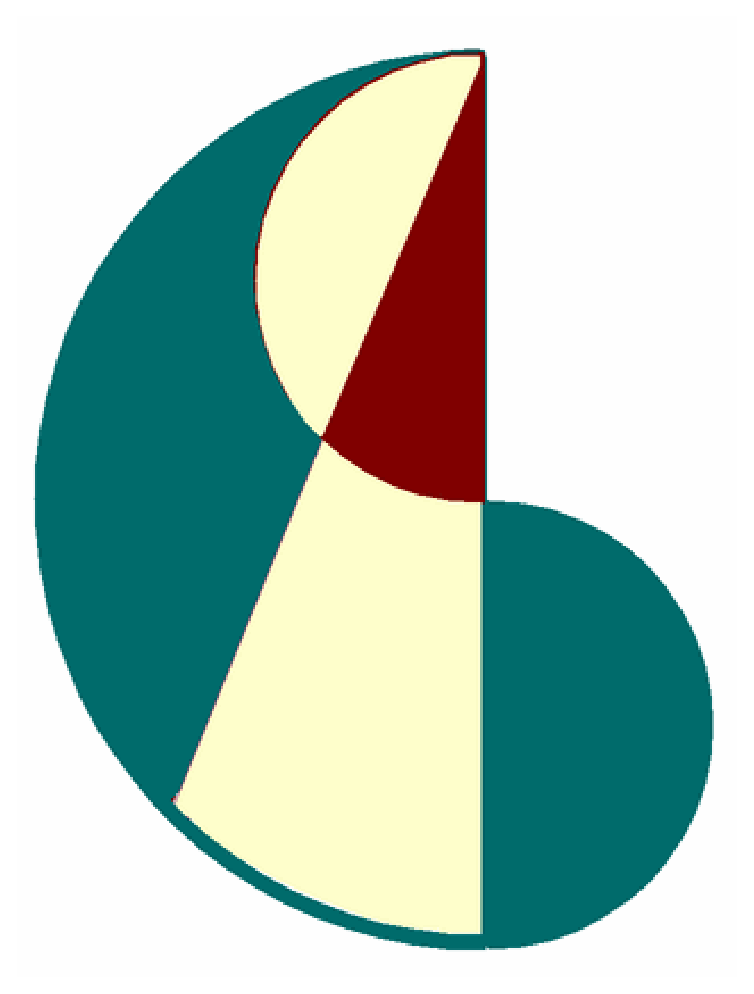
\includegraphics[width=3cm]{acstitle.eps}
\end{center}
\end{htmlonly}

\bigskip\bigskip\bigskip


\begin{center}
% lggr -> Large
% lr -> large
\begin{tabular}{llllllll}
& {\LARGE Piet Hut} & {\LARGE \&} & & & & & {\LARGE Jun Makino}\\
&  & & & & & & \\
& {\large Institute for Advanced Study} & & & & & &
  {\large Univ. of Tokyo, \ Dept. of Astronomy}\\
& {\large 1 Einstein Drive} & & & & & & {\large 7-3-1 Hongo, Bunkyo-ku}\\
& {\large Princeton, NJ 08540} & & & & & & {\large Tokyo 113-0033}\\
& {\large U.S.A.} & & & & & & {\large JAPAN}\\
& {\large piet@ias.edu} & & & & & & {\large makino@astron.s.u-tokyo.ac.jp}\\
\end{tabular}

\bigskip\bigskip\bigskip\bigskip

\end{center}
         % input, in order to let the time stamp appear
%
% uncomment the following three lines, if you want to print two pages
% on one, using e.g. "psnup -2 v1.ps > v1_2.ps".  Normally the next three
% lines should be commented out, but in that case psnup will print the right
% (left) pages on the left (right) side.
%
%\newpage
%\thispagestyle{empty}
%\mbox{}
%
    \newpage           % blank page, to force preface to start on a right hand page
\thispagestyle{empty}      % suppresses page numbering of the blank second page
\mbox{}                    % dummy content; otherwise \newpage has no effect
\newpage                   % on to third page, to start the preface
\pagenumbering{roman}      % with a roman numbering system, starting here at i

%%\chapter{Preface} %% this replace the four lines below, but at the
                    %% cost (currently) of two extra pages

\addcontentsline{toc}{chapter}{Preface}

\begin{center}
{\lgb Preface}
\end{center}

The {\it Pure Gravity} book series, of which this is the second volume,
\dots\dots\dots

%\bigskip
%\bigskip
%{\it Acknowledgments:}
%xxx
%We thank xxx, xxx and xxx for valuable
%discussions.  This work is supported in part by the Research for the
%Future Program of Japan Society for the Promotion of Science
%(JSPS-RFTP97P01102).

\tableofcontents

\listoffigures


  \mainmatter
      \chapter{The Universe in a Computer}

\section{Gravity}

Gravity is the weakest of all fundamental forces in physics, far
weaker than electromagnetism or the so-called weak and strong
interactions between subatomic particles.  However, the other three
forces lose out in the competition with gravity over long distances.
The weak and strong interactions both have an intrinsically short
range.  Electromagnetism, while being long-range like gravity, suffers
from a cancellation of attraction and repulsion in bulk matter, since
there tend to be as almost exactly as many positive as negative
charges in any sizable piece of matter.  In contrast, gravitational
interactions between particles are always attractive.  Therefore, the
larger a piece of matter is, the more gravitational force it exerts on
its surroundings.

This dominance of gravity at long distances makes the job of
modeling a chunk of the Universe easier.  To a first approximation, it
is often a good idea to neglect the other forces, and to model the
objects as if they were interacting only through gravity.  In many
cases, we can also neglect the intrinsic dimensions of the objects,
treating each object as a point in space with a given mass.  All this
greatly simplifies the mathematical treatment of a system, by leaving
out most of the physics and chemistry that would be needed in a more
accurate treatment.

This book is the first in a series of books titled {\it Pure Gravity}, to
indicate that we are making this approximation of treating objects as
gravitating masses and nothing more.  The objects we will be studying
are stars, and the environment we will focus on are dense stellar
systems, where the stars are so close together that they will
occasional collide and in general have frequent interesting and
complex interactions.  In a later series, {\it Applied Gravity}, we will
look at the internal physics of those stars: how they evolve under the
influence of nuclear reactions in their centers, how they may die in
cosmic explosions, and what happens to their remnant cores.  We will
especially study how interactions between stars of all types can change
their evolutionary behavior through two-body, three-body, and more
complex interactions, leading to an intricate `star cluster ecology'.

This first book, {\it Writing an N-Body Code}, lays the groundwork for
modeling a system of stars.  We start absolutely from scratch, with a
most simple code of less than a page long.  In many small steps we
then improve that code, pointing out the many pitfalls along the way,
on the level of programming as well as astrophysical understanding.
We introduce helpful code development facilities and give many hints as
to how to balance simplicity, efficiency, clarity, and modularity of
the code.  Our intention is to introduce the topic from square one,
and then to work our way up to a robust set of codes with which one
can do actual research.  In later volumes in this series, we will
continue to develop these codes, adding many useful diagnostic tools,
and integrating those in a full production-level software environment.

\section{Galactic Suburbia}

The sun is a star like any other among the hundred billion or so stars
in our galaxy.  It is unremarkable in its properties.  Its mass is in
the mid range of what is normal for stars: there are others more than
ten times more massive, and there are also stars more ten times less
massive, but the vast majority of stars have a mass within a factor
ten of that of the sun.  Our home star is also unremarkable in its
location, at a distance of some thirty thousand light years from the
center of the galaxy.  Again, the number of stars closer to the center
and further away from the center are comparable.  Our closest neighbor,
Proxima Centauri, lies at a distance of a bit more than four light years.

This distance is typical for separations between stars in our neck of
the woods.  A light year is ten million times larger than the diameter
of the sun (a million km, or three light seconds).  In a scale model,
if we would represent each star as a cherry, an inch across, the
separation between the stars would be many hundreds of miles.  It is
clear from these numbers that collisions between stars in the solar
neighborhood must be very rare.  Although the stars follow random
orbits without any traffic control, they present such tiny targets
that we have to wait very long indeed in order to witness two of them
crashing into each other.  A quick estimate tells us that the sun has
a chance of hitting another star of less than $10^{-18}$ per year.  In
other words, we would have to wait at least $10^{18}$ years to have an
appreciable chance to witness such a collision.  Given that the sun is
less than five billion years old, it is no surprise that it does not
show any signs of a past collision: the chance that that would have
happened was less than one in a hundred million.  Life in our galactic
suburbs is really quite safe for a star.

There are other places in our galaxy that are far more crowded, and
consequently are a lot more dangerous to venture into.  We will have
a brief look at four types of crowded neighborhoods.

\section{Globular Clusters}

\begin{figure}[ht]
\begin{center}
\epsfxsize = 4.5in
\epsffile{chap1/m15.eps}
\caption[A snapshot of the globular cluster M15]
{A snapshot of the globular cluster M15, taken with the Hubble Space
Telescope.}
\label{fig:m15}
\end{center}
\end{figure}
%%  From: http://oposite.stsci.edu/pubinfo/PR/2000/25/content/0025y.jpg

In Fig. \ref{fig:m15} we see a picture of the globular cluster M15,
taken with the Hubble Space Telescope.  This cluster contains roughly
a million stars.  In the central region typical distances between
neighboring stars are only a few hundredth of a light year, more than
a hundred times smaller than those in the solar neighborhood.  This
implies a stellar density that is more than a million times larger
than that near the sun.  Since the typical relative velocities of
stars in M15 are comparable to that of the sun and its neighbors, a
few tens of km/sec, collision times scale with the density, leading to
a central time between collisions of less than $10^{12}$ years.  With
globular clusters having an age of more than $10^{10}$ years, a typical
star near the center already has a chance of more than a percent to
have undergone a collision in the past.  

In fact, the chances are much higher than this rough estimate indicates.
One reason is the stars spend some part of their life time in a much
more extended state.  A star like the sun increases its diameter by
more than a factor of one hundred toward the end of its life, when
they become a red giant.  By presenting a much larger target to other
stars, they increase their chance for a collision during this stage
(even though this increase is partly offset by the fact that the red
giant stage lasts shorter than the so-called main-sequence life time
of a star, during which they have a normal appearance and diameter).
The other reason is that many stars are part of a double star system,
a type of dynamic spider web that can catch a third star, or another
double star, into a temporary three- or four-body dance.  Once engaged
in such a dance, the local stellar crowding is enormously enhanced,
and the chance for collisions is greatly increased. 

A detailed analysis of all these factors predicts that a significant
fraction of stars in the core of a dense globular cluster such as M15
has already undergone at least one collision in its life time.  This
analysis, however, is quiet complex.  To study all of the important
channels through which collisions may occur, we have to analyze
encounters between a great variety of single and double stars, and
occasional bound triples and larger bound multiples of stars.  Since
each star in a bound subsystem can be a normal main-sequence star, a
red giant, a white dwarf, a neutron star or even a black hole, as well
as an exotic collision product itself, the combinatorial richness of
flavors of double stars and triples is enormous.  If we want to pick a
particular double star, we not only have to choose a star type for
each of its members, but in addition we have to specify the mass of
each star, and the parameters of its orbit, such as the semimajor axis
(a measure for the typical separation of the two stars) as well as the
orbital eccentricity.

The goal of our book series is to develop the software tools to make
it possible to simulate an entire star cluster like M15, and to
analyze the resulting behavior both locally and globally.

\clearpage  % to let the m15 picture be inserted not further than here

\section{Galactic Nuclei}

In Fig. \ref{fig:gc} we see an image of the very center of our galaxy.
This picture is taken with the Northern branch of the two Gemini
telescopes, which is located in Hawaii on top of the mountain Mauna Kea.

\begin{figure}[ht]
\begin{center}
\epsfxsize = 4.5in
\epsffile{chap1/gc.eps}
\caption[An image of the central region of our galaxy]
{An image of the central region of our galaxy, taken with the Gemini
North telescope.  The center is located on the right just above the
bottom edge of the image.}
\label{fig:gc}
\end{center}
\end{figure}
%% From: http://www.gemini.edu/gallery/observing/gc\_color.jpg

In the very center of our galaxy, a black hole resides with a mass
a few million times larger than the mass of our sun.  Although the
black hole itself is invisible, we can infer its presence by its
strong gravitational field, which in turn is reflected in the speed
with which stars pass near the black hole.  In normal visible light it
is impossible to get a glimpse of the galactic center, because of the
obscuring gas clouds that are positioned between us and the center.
Infrared light, however, can penetrate deeper in dusty regions.
Fig. \ref{fig:gc} is a false-color image, reconstructed from
observations in different infrared wavelength bands.

In the central few light years near the black hole, the total mass of
stars is comparable to the mass of the hole.  This region is also
called the galactic nucleus.  Here the stellar density is at least as
large as that in the center of the densest globular clusters.  However,
due to the strong attraction of the black hole, the stars zip around at
much higher velocities.  Whereas a typical star in the core of M15 has
a speed of a few tens of km/sec, stars near the black hole in the
center of our galaxy move with speeds exceeding a 1000 km/sec.  As a
consequence, the frequency of stellar collisions is strongly enhanced.

Modeling the detailed behavior of stars in this region remains a great
challenge, partly because of the complicated environmental features.
A globular cluster forms a theorist's dream of a laboratory, with its
absence of gas and dust and starforming regions.  All we find there
are stars that can be modeled well as point particles unless they come
close and collide, after which we can apply the point particle
approximation once again.  In contrast, there are giant molecular
clouds containing enormous amounts of gas and dust right close up to
the galactic center.  In these clouds, new stars are formed, some of
which will soon afterwards end their life in brilliant supernova
explosions, while spewing much of their debris back into the
interstellar medium.  Such complications are not present in globular
clusters, where supernovae no longer occur since the member stars are
too old and small to become a supernova.

Most other galaxies also harbor a massive black hole in their nuclei.
Some of those have a mass of hundreds of millions of solar masses, or
in extreme cases even more than a billion times the mass of the sun.
The holy grail of the study of dense stellar systems is to perform and
analyze accurate simulations of the complex ecology of stars and gas
in the environment of such enormous holes in space.  Much of the
research on globular clusters can be seen as providing the initial
steps toward a detailed modeling of galactic nuclei.

\section{Star Forming Regions}

\begin{figure}[ht]
\begin{center}
\epsfxsize = 3in
\epsffile{chap1/orion.eps}
\caption[The Orion Nebula]
{The Orion Nebula, as seen by the Subaru telescope.}
\label{fig:orion}
\end{center}
\end{figure}
%%  From: http://www.subaru.naoj.org/Science/press\_release/9901/Orion.jpg

There are many other places in the galactic disk where the density of
stars is high enough to make collisions likely, at least temporarily.
These are the sites where stars are born.  Fig. \ref{fig:orion} taken
by the Japanese Subaru telescope in Hawaii shows the Orion Nebula,
also known as M42, at a distance of 1500 light years from the sun.
This picture, too, is taking in infrared light in order to penetrate
the dusty regions surrounding the young stars.  The four brightest
stars in the center, collectively known as the Trapezium, form the
most massive stars of a larger conglomeration of stars, all recently
formed from the gas and dust that still surrounds them.

In order to study collisions in these star forming regions, we can no
longer treat the stars are point masses.  Many of the collisions take
place while the stars are still in the process of forming.  While a
protostar is still in the process of contracting from the gas cloud
in which it was born, it presents a larger target for collisions with
other stars.  In addition, a single contracting gas cloud may fission,
giving rise to more than one star at the same time.  In this way, the
correlated appearance of protostars is even more likely to lead to
subsequent collisions.

The proper way to model these processes is to combine gas dynamics and
stellar dynamics.  Much progress has been made recently in this area.
One way to use stellar dynamics in an approximate fashion is to begin
with the output of the gas dynamics codes, which present the positions
and velocities of a group of newly formed stars, and then to follow
and analyze the motions of those stars, including their collisions.

\section{Open Clusters}

Although stars are formed in groups, these groups typically do not
stay together for very long.  Perturbations from other stars and gas
clouds in their vicinity are often enough to break up the fragile
gravitational hold they initial have over each other.  Some of the
more massive groups of newly formed stars, however, are sufficiently
tightly bound to survive their environmental harassment.  They form
the so-called open clusters, where there name indicates that they have
central densities that are typically less than what we see in globular
clusters.

\begin{figure}[ht]
\begin{center}
\epsfxsize = 2.5in
\epsffile{chap1/m67.ps}
\caption[The open star cluster M67]
{The open star cluster M67, in a picture taken by the Anglo-Australian
Observatory.}
\label{fig:m67}
\end{center}
\end{figure}
%%  From: http://www.seds.org/messier/Pics/More/m67aat.jpg

Fig. \ref{fig:m67} shows one of the richest and densest open clusters,
M67, as observed by the Anglo-Australian Observatory.  Since this
cluster is old enough to have lost its gas and dust, all stars are
visible at normal optical wavelengths, at which this image is taken.
In the central regions of this cluster, there are indications that
some of the stars have undergone close encounters or even collisions.
Consequently, this star cluster qualifies as a dense stellar system.

Open clusters typically have fewer members than globular clusters.
Also, they are younger.  Both facts makes it easier to simulate open
clusters than globular clusters.  On the other hand, the densest
globular clusters show a higher frequency and a far richer variety of
stellar collisions, making them a more interesting laboratory.  In
that sense, a dynamical simulation of an open cluster can be seen as
providing preparatory steps toward the modeling of globular clusters,
just as a study of the latter forms a stepping stone toward the
investigation of galactic nuclei.

\section{Writing your own star cluster simulator}

Astronomers have almost half a century of experience in writing
computer codes to simulate dense stellar systems.  The first published
results date back to 1960, and it was in the subsequent decade that it
became clear just how tricky it was to simulate a group of interacting
stars.  The task seems so easy: just integrate Newton's equations of
motion for each star, under the influence of the gravitational pairwise
interactions of all other stars.  Indeed, it is straightforward to
write a simple code to do so, as we will see below.  And as long as
all stars remain fairly well separated from each other, even a simple
code will do a reasonably good job.

In practice, though, even a small group of stars will spontaneously
form one or more double stars.  This was discovered experimentally in
the early sixties.  One way to understand this result, after the fact,
is from an energetic point of view.  When a double star, or binary as they
are generally called, is formed, energy is released.  Since the two stars
in a binary are bound, the potential energy is larger than the kinetic
energy, and the total energy is negative.  When three stars come together
randomly, there is a chance that two of the three are left in a bound
state, while the third one escapes, carrying the excess energy.  Left
by itself, a stellar system will exploit this energy liberation
mechanism by spontaneously forming binaries.

As soon as even one binary appears, a simple code with constant time
steps will either crash or resort to a very slow and inefficient crawl.
The changes in the relative configuration of the two stars occur so
frequent that they can be easily missed.  If they are modeled correctly,
by choosing a tiny time step, the rest of the system will be forced to
slow down, while spending a large and unnecessary amount of computer
time on all the other stars that don't need such fine resolution.  By
the end of the sixties, these problems were overcome by the development
of codes that employed individual time steps.  Stars with close
neighbors were stepped forward in time more frequently than stars at
large, and in this way the computational power was brought to where it
was most needed.

This modification in itself brought gravitational $N$-body codes already
well outside the range of systems that are normally discussed in text
books on numerical integration methods.  The internal book keeping
needed to write a correct and efficient code with individual time
steps is surprisingly large, given the simplicity of the task:
integrate the effect of pairwise attractive inverse square forces.
But this was only a first step toward the development of modern $N$-body
codes.  The presence of tight binaries produced much more of an obstacle,
and throughout the seventies a variety of clever mechanisms were developed
in order to deal with them efficiently.

For one thing, there are problems with round-off.  Two stars in a tight
orbit around each other have almost the same position vector, as seen
from the center of a star cluster, where we normally anchor the global
coordinate system.  And yet it is the separation between the stars
that determines their mutual forces.  When we compute the separation
by subtracting two almost identical spatial vectors, we are asking for
(numerical) trouble.  The solution is to introduce a local coordinate
system whenever two or more stars undergo a close interaction.  This
does away with the round-off problem, but it introduces a host of
administrative complexities, in order to make sure that any arbitrary
configuration of stars is locally presented correctly -- and that the
right thing happens when two or more of such local coordinate patches
encounter each other.  This may not happen often, but one occurrence
in a long run is enough to crash the system if no precautions have
been taken for such a situation to happen.

We can continue the list of tricks that have been invented to allow
every larger and denser systems to be modeled correctly.  Numerical
problems with the singularity in the two-body system have been
overcome by mapping two or more interacting stars from the
three-dimensional Kepler problem to a four-dimensional harmonic
oscillator.  The total force on particles has been split into
different contributions, the first from a near zone of relatively
close neighbors and the second from a far zone of all other particles,
with each partial force being governed with different integration time
steps.  Tree codes have been used to group the contributions of a
number of more and more distant zones together in ever larger chunks,
for efficiency.  Triple stars have received their own special treatment,
especially the marginally stable triples that are sometimes long-lived, 
but continuously changed their inner state due to internal perturbations.
The list goes on.

In this first book, we will introduce a modern integrator, the Hermite
scheme, developed in the 1990s, together with a variable time step
integration scheme, where all stars share a common time step at any
given time.  In subsequent volumes in the series, we will introduce
the other refinements mentioned above.  Our emphasis will be on a
complete explanation of all the steps involved, together with a
discussion of the motivation for those steps.  In the last few
chapters, we will embark on a research project featuring stellar
collisions, in a simple gravity-only approximation.

    \part{Object Oriented $N$-Body Codes}
      \chapter{A Shared Time Step Code with Class(es)}


      \chapter{A Code with Individual Time Steps}


    \part{Mini Gravitylab}
      \chapter{A Topological Investigation of Parameter Space}


      \chapter{Automatization of Laboratory Experiments}


    \part{Astrophysical Applications}
      \chapter{Exploring $N = 3$ with a Hermite Algorithm}

Having seen the dramatic improvement that came from switching from the
forward Euler algorithm to the leapfrog, the obvious next step was to
go to yet higher order algorithms.  A quick look in a few books of
numerical methods showed our friends that there was a bewildering
choice of third- and fourth-order methods to choose from.  Alice then
mentioned that her thesis advisor had pointed her to an elegant and
natural generalization of the leapfrog algorithm, by the name of the
Hermite scheme.

\section{A Surprisingly Simple Hermite Scheme}

The most symmetric Hermite version, and the one closest resembling the
leapfrog is this one:

\def\half{{\textstyle\frac{1}{2}}}
\def\quarter{{\textstyle\frac{1}{4}}}
\def\one#1{{\textstyle\frac{1}{#1}}}
\def\three#1{{\textstyle\frac{3}{#1}}}
\def\seven#1{{\textstyle\frac{7}{#1}}}

\begin{eqnarray}
\br_{i+1} & = & \br_i + \half(\bv_i + \bv_{i+1}) dt +
                \one{12}(\ba_i - \ba_{i+1})(dt)^2
                \label{hermite-step1} \\
\bv_{i+1} & = & \bv_i + \half(\ba_i + \ba_{i+1}) dt +
                \one{12}(\bj_i - \bj_{i+1})(dt)^2
                \label{hermite-step2}
\end{eqnarray}

Here $\bj = d\ba/dt$ is the {\it jerk}, the time derivative of the
acceleration, and therefore the third time derivative of position:

\begin{equation}
\bj = \frac{d^3}{dt^3} \br
\end{equation}

The term `jerk' has crept into the literature relatively recently,
probably originally as a pun.  If a car or train changes acceleration
relatively quickly you experience not a smoothly accelerating or
decelerating motion, but instead a rather `jerky' one.

The jerk can be computed through straightforward differentiation of
Newton's gravitational equations, Eq. \ref{newton}:

\begin{equation}
\bj_i =  G \sum_{j=1 \atop j \neq i}^N \,M_j \left[
\frac{\bv_{ji}}{r_{ji}^3} - 3 \frac{(\br_{ji}\cdot\bv_{ji})\br_{ji}}{r_{ji}^5}
\right]\label{newton-jerk}
\end{equation}

\noindent
where $\bv_{ji} = \bv_j - \bv_i$.

As an aside, note that the jerk has one very convenient property.
Although the expression above looks quite a bit more complicated than
Newton's original equations, they can still be evaluated through one
pass over the whole $N$-body system.  This is no longer true for
higher derivatives.  For example, we can obtain the fourth derivative
of the position of particle $i$ (the {\it snap}, see next section) by
differentiating Eq. \ref{newton-jerk}:

\begin{eqnarray}
\frac{d^4}{dt^4}\br_i = G \sum_{j=1 \atop j \neq i}^N \,M_j \Bigg[ &\,&
\!\!\!\!\!\!\!\!\!\! \frac{\ba_{ji}}{r_{ji}^3}
-6 \frac{(\br_{ji}\cdot\bv_{ji})}{r_{ji}^5}\bv_{ji} \nonumber \\
 &\,& \!\!\!\!\!\!\!\! + \left\{ -3\frac{v_{ji}^2}{r_{ji}^5}
-3 \frac{(\br_{ji}\cdot\ba_{ji})}{r_{ji}^5}
+15 \frac{(\br_{ji}\cdot\bv_{ji})^2}{r_{ji}^7} \right\} \br_{ji} \,\,\Bigg]
\label{newton-snap}
\end{eqnarray}

\noindent
where $\ba_{ji} = \ba_j - \ba_i$, and this is the expression that
thickens the plot.  Unlike the $\br_{ji}$ and $\bv_{ji}$ expressions,
that are given by the initial conditions, $\ba_{ji}$ has to be
calculated from the positions and velocities.  However, this
calculation does not only involve the pairwise attraction of particle
$j$ on particle $i$, but in fact all pairwise attractions of all
particles on each other!  This follows immediately when we write out
what the shorthand implies:

\begin{equation}
\ba_{ji} = \ba_j - \ba_i = G \sum_{k=1 \atop k \neq j}^N
\frac{M_k}{r_{kj}^3} \,\br_{kj} -  G \sum_{k=1 \atop k \neq i}^N
\frac{M_k}{r_{ki}^3} \,\br_{ki}
\end{equation}

\noindent
When we substitute this back into Eq. \ref{newton-snap}, we see that
we have to do a double pass over the $N$-body system, summing over
both indices $k$ and $j$ in order to compute a single fourth derivative
for the position of particle $i$.  

\section{Comparison with the Leapfrog}

When we look at Eqs. \ref{hermite-step1}, \ref{hermite-step2}, we see
some familiar features.  Neglecting the higher-order term for the
moment, we recognize the leapfrog: the new position is effectively
determined by the mid-point velocity $v_{i+1/2}$, here approximated as
the average between the two adjacent values $v_{i}$ and $v_{i+1}$.
Similarly, the new velocity is effectively determined by the mid-point
acceleration.

In fact, the analogy can be made more precise.  Recalling the leapfrog,
as written centered on integer times, Eqs. \ref{leapfrog-step1},
\ref{leapfrog-step2}:

\begin{eqnarray}
\br_{i+1} & = & \br_i + \bv_{i} dt + \ba_{i} (dt)^2/2 \label{leapfrog-step1a}\\
\bv_{i+1} & = & \bv_i + (\ba_i + \ba_{i+1})dt / 2 \label{leapfrog-step2a}
\end{eqnarray}

\noindent
we can transform these back into a pseudo-leap form, without using
half-integer times explicitly, by rewriting the first equation as:

\begin{eqnarray}
\br_{i+1} & = & \br_i + \half(\bv_{i} + \bv_{i+1}) dt
                      + \half(\bv_{i} - \bv_{i+1}) dt
                      + \half\ba_{i} (dt)^2 \nonumber \\
	  & = & \br_i + \half(\bv_{i} + \bv_{i+1}) dt
                      + \quarter(-\ba_i-\ba_{i+1})(dt)^2
                      + \half\ba_{i}(dt)^2 \nonumber \\
	  & = & \br_i + \half(\bv_{i} + \bv_{i+1}) dt
                      + \quarter(\ba_i-\ba_{i+1})(dt)^2 \nonumber \\
	  & = & \br_i + \half(\bv_{i} + \bv_{i+1}) dt - \quarter\bj_i (dt)^3
                                                      \label{leapfrog-trick}
\end{eqnarray}

In the second line, we have simply rearranged terms.  In the third
line, we have used \ref{leapfrog-step2a}, and in the fourth line we
have used the definition of $\bj$, while neglecting higher order terms
in $dt$.

The next step is to remember that the leapfrog is a second-order scheme.
The errors per step are $\propto(dt^3)$, and therefore it does not
matter whether or not we include the last term $-\bj_i (dt)^3/4$ into
our leapfrog version: this term is lost in the noise, and is not going
to improve the accuracy on second-level order.  Therefore, we may
equally well leave it out.  Doing so transforms Eqs. \ref{leapfrog-step1a},
\ref{leapfrog-step2a} into:

\begin{eqnarray}
\br_{i+1} & = & \br_i + \half(\bv_i + \bv_{i+1})dt \label{leapfrog-step1b} \\
\bv_{i+1} & = & \bv_i + \half(\ba_i + \ba_{i+1})dt \label{leapfrog-step2b}
\end{eqnarray}

Here we see explicitly that our good old leapfrog is equivalent, up to
its second-order accuracy, with the leading terms $\propto (dt)$ of
the Hermite algorithm, Eqs. \ref{hermite-step1}, \ref{hermite-step2}.
It is a curiosity of the leapfrog that at first sight it resembles a
first-order scheme, since the second-order terms are hidden in the
`leapy' way of using average quantities.  Yet, as we have seen, the
leapfrog is fully second-order.

In a very similar way, the Hermite scheme is fourth-order, even though
it resembles a second-order scheme.  For details we refer to the
literature, but it is interesting to see in a heuristic way why this
is so.

\section{Snap, Crackle, and Pop}

First a word about terminology.  We will need to introduce a few extra
derivatives of the position.  It would be fun to give them names with
a reasonable `feel' to them, just like with jerk.  What type of motion
feels even more restless than jerking motion?  A sudden snap comes to
mind.  A what changes its state more sudden than a snap --- how about
a crackle?  And for those familiar with American rice crispies culture,
a pop cannot be far away, and indeed, if something pops it really
changes high derivatives of positions in a substantial way!  We are
not making these names up: we have seen them used a few times before,
although the precise source is likely to be lost in (recent) history.
So here they are:

\begin{equation}
\bs = \frac{d^4}{dt^4} \br \qquad ; \qquad
\bc = \frac{d^5}{dt^5} \br \qquad ; \qquad
\bp = \frac{d^6}{dt^6} \br
\end{equation}

\noindent
{\it snap}, {\it crackle}, and {\it pop}, respectively.

We are now in a position to write the Taylor series for the four
quantities that appear in Eqs. \ref{hermite-step1}, \ref{hermite-step2},
up to crackle:

\begin{eqnarray}
\br_{i+1} & = & \br_i + \bv_i dt + \half\ba_{i}(dt)^2 + \one{6}\bj_{i}(dt)^3
                      + \one{24}\bs_{i}(dt)^4 + \one{120}\bc_{i}(dt)^5
                                                           \label{taylor-r} \\
\bv_{i+1} & = & \bv_i + \ba_i dt + \half\bj_{i}(dt)^2 + \one{6}\bs_{i}(dt)^3
                      + \one{24}\bc_{i}(dt)^4              \label{taylor-v} \\
\ba_{i+1} & = & \ba_i + \bj_i dt + \half\bs_{i}(dt)^2 + \one{6}\bc_{i}(dt)^3
                                                           \label{taylor-a} \\
\bj_{i+1} & = & \bj_i + \bs_i dt + \half\bc_{i}(dt)^2      \label{taylor-j}
\end{eqnarray}

\noindent
We can now eliminate snap and crackle at time $t_i$, expressing them
in terms of the acceleration and jerk at times $t_i$ and $t_{i+1}$,
using Eqs. \ref{taylor-a}, \ref{taylor-j}.  We find:

\begin{eqnarray}
\bs_i &=& -6\ba_i +6\ba_{i+1} -4\bj_i -2\bj_{i+1} \\
\bc_i &=& 12\ba_i -12\ba_{i+1} +6\bj_i +6\bj_{i+1} 
\end{eqnarray}

\noindent
Substituting both expressions in Eq. \ref{taylor-v} we directly find:

\begin{equation}
\bv_{i+1} = \bv_i + \half(\ba_i + \ba_{i+1}) dt +
                \one{12}(\bj_i - \bj_{i+1})(dt)^2 \label{hermite-step2a}
\end{equation}

\noindent
Indeed, we have recovered Eq. \ref{hermite-step2}, and thereby
explained the mysterious factor $\one{12}$ in the last term.

Let us complete our mission, by making the same derivation for 
the position vector, Eq. \ref{hermite-step1}, in the Hermite scheme.
Using again the snap and crackle expressions derived above, we find:

\begin{equation}
\br_{i+1} = \br_i + \bv_i dt + (\seven{20}\ba_i + \three{20}\ba_{i+1})(dt)^2
            + (\one{20}\bj_i - \one{30}\bj_{i+1})(dt)^3
\end{equation}

\noindent
Using the same trick we employed in Eq. \ref{leapfrog-trick} to factor
out the velocity terms, and using Eq. \ref{hermite-step2a}, we can
rewrite the above expression as:

\begin{equation}
\br_{i+1} = \br_i + \half(\bv_i + \bv_{i+1}) dt
            + \one{10}(\ba_i - \ba_{i+1})(dt)^2
            + \one{120}(\bj_i + \bj_{i+1})(dt)^3
\end{equation}

\noindent
While this result still looks quite different from Eq. \ref{hermite-step1},
we claim that it is identical up to fourth-order in $dt$, which is all we
need.  Our final step thus parallels the discussion following
Eq. \ref{leapfrog-trick} for the leapfrog, where we had to show how
terms up to second-order were identical.

First we rewrite the above equation in terms of quantities defined at $t=i$:

\begin{eqnarray}
\br_{i+1} = \br_i + \half(\bv_i + \bv_{i+1}) dt 
             & + & \one{10}\ba_i(dt)^2 - \one{10}(\ba_i + \bj_i dt +
              \half\bs_i (dt)^2)(dt)^2                           \nonumber \\
          & + & \one{120}\bj_i(dt)^3 + \one{120}(\bj_i + \bs_i dt)(dt)^3
                                                                 \nonumber \\
          = \br_i + \half(\bv_i + \bv_{i+1}) dt 
          & - & \one{12}\bj_i (dt)^3 - \one{24} \bs_i (dt)^4
\end{eqnarray}

\noindent
Here we have left out terms containing $\bc_i$, since they would be
proportional to at least $(dt^5)$ and only contribute to the error noise.
We can similarly write out the last term of Eq. \ref{hermite-step1}:

\begin{eqnarray}
\one{12}(\ba_i - \ba_{i+1})(dt)^2  & = & 
              \one{12}\left(\ba_i(dt)^2 - \one{12}(\ba_i + \bj_i dt +
              \half\bs_i (dt)^2)\right)(dt)^2                     \nonumber \\
             & = & - \one{12}\bj_i (dt)^3 - \one{24} \bs_i (dt)^4
\end{eqnarray}

\noindent
This proves the desired result:

\begin{equation}
\br_{i+1} = \br_i + \half(\bv_i + \bv_{i+1}) dt +
                \one{12}(\ba_i - \ba_{i+1})(dt)^2
\end{equation}

\section{Implementing Hermite}

Let us return to Alice, Bob, and Carol, who are about to implement the
Hermite scheme.  Since Bob was most eager to test out this new
algorithm, he got his turn behind the computer.

\abc

\bob
Let's give this new Hermite scheme a stress test.  I'll take {\st
leapfrog2a.C}, the one with the off-set in initial velocity of
$10^{-4}$, call it {\st hermite1a.C} for now, and simply substitute
the leapfrog equations \ref{leapfrog-step1}, \ref{leapfrog-step2} by
the Hermite equations \ref{hermite-step1}, \ref{hermite-step2}.

\carol
Why not call the code {\st hermite1.C}?

\bob
Even though the update seems almost trivial, I don't have the audacity
to believe we'll get everything right the first time around.  When it
all works, we will rename the code to {\st hermite1.C}.  So here is
the new version:

\cba

\code{hermite1a.C}{chap6/hermite1a.C}

\abc

\alice
Ah, I see now that you were wise giving the code an preliminary name.
Notice where you have added the jerk calculation.  You replaced

\begin{small}
\begin{verbatim}
            for (int k = 0; k < 3; k++){
                a[i][k] += m * rji[k] / r3;
                a[j][k] -= m * rji[k] / r3;
            }
\end{verbatim}
\end{small}

\noindent
by:

\begin{small}
\begin{verbatim}
            for (int k = 0; k < 3; k++){
                a[i][k] += m * rji[k] / r3;
                a[j][k] -= m * rji[k] / r3;
                jk[i][k] += m * (vji[k] - 3 * rv * rji[k]) / r3;
                jk[j][k] -= m * (vji[k] - 3 * rv * rji[k]) / r3;
            }
\end{verbatim}
\end{small}

\noindent
in addition to some extra changes, such as introducing and calculating
the variable {\st vji[]} for the relative velocities for particles $i$
and $j$.  All of this is fine, as far as I can see.  The statements are
correctly written and reflect the Hermite, but there is one problem.
In the last two lines above you use the relative velocities $vij[]$,
but at this point in the program they have not been assigned yet.

\bob
Ah, you are right.  That happens just a few lines below, with this
`clever' trick of using the magnitude of the centrifugal acceleration
to determine the magnitude of the velocities.  Thanks!  Okay, so I'll
make another version, {\st hermite1b.C}, which has two initial loops,
one for the accelerations, followed by the assignment of velocities,
and then followed by the second loop which computes the jerks.

\carol
Maybe we can just run the program using our friend {\st /dev/null} to
see how the energy behaves, before start making pictures.  I'm really
curious to see whether we have now reached fourth-order accuracy.

\bob
Easy to test:

\cba

\begin{small}
\begin{verbatim}
|gravity> g++ -o hermite1b hermite1b.C
|gravity> hermite1b > /dev/null
Please provide a value for the time step
0.01
and for the duration of the run
100
Initial total energy E_in = -0.866025
Final total energy E_out = -0.975389
absolute energy error: E_out - E_in = -0.109364
relative energy error: (E_out - E_in) / E_in = 0.126282
|gravity> !!
hermite1b > /dev/null
Please provide a value for the time step
0.001
and for the duration of the run
100
Initial total energy E_in = -0.866025
Final total energy E_out = -0.866586
absolute energy error: E_out - E_in = -0.000560173
relative energy error: (E_out - E_in) / E_in = 0.000646832
|gravity> !!
hermite1b > /dev/null
Please provide a value for the time step
0.0001
and for the duration of the run
100
Initial total energy E_in = -0.866025
Final total energy E_out = -0.866026
absolute energy error: E_out - E_in = -5.52839e-07
relative energy error: (E_out - E_in) / E_in = 6.38364e-07
|gravity> !!
hermite1b > /dev/null
Please provide a value for the time step
0.00001
and for the duration of the run
100
Initial total energy E_in = -0.866025
Final total energy E_out = -0.866025
absolute energy error: E_out - E_in = -5.53711e-10
relative energy error: (E_out - E_in) / E_in = 6.39371e-10
|gravity> 
\end{verbatim}
\end{small}

\abc

\carol
What is this?  We seem to have constructed a third-order algorithm!

\alice
Hmmm.  It seems that way.  Each refinement of a factor ten in step
size gives a reduction of the error of a factor 1000.  But this was
not supposed to happen

\bob
This is strange indeed.  Look, at the end, there they are, the real
Hermite expressions, what can be wrong with such simple statements??

\begin{small}
\begin{verbatim}
        for (int i = 0; i < n; i++){
            for (int k = 0; k < 3; k++){
                r[i][k] = old_r[i][k] + (old_v[i][k] + v[i][k])*dt/2
                                      + (old_a[i][k] - a[i][k])*dt*dt/12;
                v[i][k] = old_v[i][k] + (old_a[i][k] + a[i][k])*dt/2
                                      + (old_j[i][k] - jk[i][k])*dt*dt/12;
            }
        }
\end{verbatim}
\end{small}

\carol
Yes, they are just what we derived before, as Eqs. \ref{hermite-step1},
\ref{hermite-step2}.

\alice
Could we have made a similar mistake as we did just before, when the
expressions were absolutely correct, but the order of execution was wrong?

\bob
Well \dots hmmm \dots aha, of course, you are right!  Look, that is
exactly the problem.  In the first line, where the position is updated,
we indicate that we are using both the old velocity values and the new
velocity values.  However, the new ones have not been computed yet ---
that happens only on the next line!  And the solution is obvious:
fortunately, the second line updating the velocity does not have this
problem, since it uses only accelerations and jerks, all of which have
already been computed, both for the old and the new values.  So we can
simply swap the lines, and this should now work:

\begin{small}
\begin{verbatim}
        for (int i = 0; i < n; i++){
            for (int k = 0; k < 3; k++){
                v[i][k] = old_v[i][k] + (old_a[i][k] + a[i][k])*dt/2
                                      + (old_j[i][k] - jk[i][k])*dt*dt/12;
                r[i][k] = old_r[i][k] + (old_v[i][k] + v[i][k])*dt/2
                                      + (old_a[i][k] - a[i][k])*dt*dt/12;
            }
        }
\end{verbatim}
\end{small}

\section{Testing the Hermite: Three Stars on a Circle}

\bob
Now I'm ready to be brave and call the code {\st hermite1.C}.  Rather
than listing the whole output, let me use the {\st diff} program,
which only lists those lines that are different.

\cba

\begin{small}
\begin{verbatim}
|gravity> diff hermite1a.C hermite1.C
2c2
< // hermite1a.C
---
> // hermite1.C
30c30
<             a[i][k] = jk[i][k] = 0.0;
---
>             a[i][k] = 0.0;
33,34c33,34
<             double rji[3], vji[3];
<             for (int k = 0; k < 3; k++){
---
>             double rji[3];
>             for (int k = 0; k < 3; k++)
36,37d35
<                 vji[k] = v[j][k] - v[i][k];
<             }
42,45d39
<             double rv = 0;
<             for (int k = 0; k < 3; k++)
<                 rv += rji[k] * vji[k];
<             rv /= r2;
49,50d42
<                 jk[i][k] += m * (vji[k] - 3 * rv * rji[k]) / r3;
<                 jk[j][k] -= m * (vji[k] - 3 * rv * rji[k]) / r3;
64a57,81
>     for (int i = 0; i < n; i++)
>         for (int k = 0; k < 3; k++)
>             jk[i][k] = 0.0;
>     for (int i = 0; i < n; i++){
>         for (int j = i+1; j < n; j++){
>             double rji[3], vji[3];
>             for (int k = 0; k < 3; k++){
>                 rji[k] = r[j][k] - r[i][k];
>                 vji[k] = v[j][k] - v[i][k];
>             }
>             double r2 = 0;
>             for (int k = 0; k < 3; k++)
>                 r2 += rji[k] * rji[k];
>             double r3 = r2 * sqrt(r2);
>             double rv = 0;
>             for (int k = 0; k < 3; k++)
>                 rv += rji[k] * vji[k];
>             rv /= r2;
>             for (int k = 0; k < 3; k++){
>                 jk[i][k] += m * (vji[k] - 3 * rv * rji[k]) / r3;
>                 jk[j][k] -= m * (vji[k] - 3 * rv * rji[k]) / r3;
>             }
>         }
>     }
> 
127,128d143
<                 r[i][k] = old_r[i][k] + (old_v[i][k] + v[i][k])*dt/2
<                                       + (old_a[i][k] - a[i][k])*dt*dt/12;
130a146,147
>                 r[i][k] = old_r[i][k] + (old_v[i][k] + v[i][k])*dt/2
>                                       + (old_a[i][k] - a[i][k])*dt*dt/12;
|gravity>
\end{verbatim}
\end{small}

\abc

\carol
Yes, that is much clearer than listing the whole source code again.
I can see how the main difference has been the move of the jerk
calculation from the earlier part, where it was entangled with the
acceleration calculation, to a separate block listed nearly at the
end.  At the very end, of course, there is the indication that we have
swapped the order of the calculations of the positions and the velocities.
The {\st diff} program arbitrarily took the velocity calculation as a
identical standard in each file, with respect to which the shift in
order of the position calculation was noted.

\alice
Soon we should start to clean up our codes, splitting them in
functions at least, and probably also in different files.  That way we
don't have to rely on {\st diff} to read our own programs, since we
can then take natural chunks at a time, in the form of functions.  But
first let's see what will happen to our figure 8 orbits.

\bob
Here are the results.  Hmm, not a very good energy conservation, if
you ask me.

\cba

\begin{small}
\begin{verbatim}
|gravity> g++ -o hermite1 hermite1.C
|gravity> hermite1 > hermite1_0.01_100.out
Please provide a value for the time step
0.01
and for the duration of the run
100
Initial total energy E_in = -0.866025
Final total energy E_out = -1.08608
absolute energy error: E_out - E_in = -0.220054
relative energy error: (E_out - E_in) / E_in = 0.254096
|gravity>
\end{verbatim}
\end{small}

\abc

\carol
Indeed.  The leapfrog did far better at this stage.  We got a relative
energy error of less than $10^{-3}$, and here we are faced with a relative
energy error of a quarter!

\alice
That is not so strange, actually.  A higher-order algorithm computes
higher-order derivatives, and therefore can be extra sensitive to
close encounters or other situations in which changes happen quite
suddenly.  Let's look at the picture, and then move on, refining our
step size.

\cba

\begin{figure}[htb]
\begin{center}
\epsfxsize = 2.5in
\epsffile{chap6/hermite1_0.01_100.ps}
\caption[Three stars on a circle, Hermite, $dv_{init}=0.0001$, $dt = 0.01$,
$t_{end} = 100$]
{The first Hermite attempt to integrate the orbits of three stars
starting off on a circle with an initial velocity perturbation of 
$dv_{init}=0.0001$, time step $dt = 0.01$ and a total duration of
$t_{end} = 100$}
\label{fig:hermite1-0.01-100}
\end{center}
\end{figure}

\begin{small}
\begin{verbatim}
|gravity> hermite1 > hermite1_0.001_100.out
Please provide a value for the time step
0.001
and for the duration of the run
100
Initial total energy E_in = -0.866025
Final total energy E_out = -0.866026
absolute energy error: E_out - E_in = -9.19142e-07
relative energy error: (E_out - E_in) / E_in = 1.06133e-06
|gravity>
\end{verbatim}
\end{small}

\begin{figure}[htb]
\begin{center}
\epsfxsize = 2.5in
\epsffile{chap6/hermite1_0.001_100.ps}
\caption[Three stars on a circle, Hermite, $dv_{init}=0.0001$, $dt = 0.001$,
$t_{end} = 100$]
{The second Hermite attempt to integrate the orbits of three stars
starting off on a circle with an initial velocity perturbation of 
$dv_{init}=0.0001$, time step $dt = 0.001$ and a total duration of
$t_{end} = 100$}
\label{fig:hermite1-0.001-100}
\end{center}
\end{figure}

\abc

\carol
Ah, much better!  Amazing.

\bob
An improvement of more than a factor 100,000 in accuracy!

\carol
And look at the picture.  I cannot see any difference between Fig. 
\ref{fig:hermite1-0.001-100} and the last picture in the series that
we did with the leapfrog, Fig. \ref{fig:leap2a-0.00001-100}!

\alice
Let's take another refinement step, to see whether we can determine
the asymptotic behavior of the error growth.  Clearly, our first
attempt was not reliable, so we need at least a third try.

\cba

\begin{small}
\begin{verbatim}
|gravity> hermite1 > hermite1_0.0001_100.out
Please provide a value for the time step
0.0001
and for the duration of the run
100
Initial total energy E_in = -0.866025
Final total energy E_out = -0.866025
absolute energy error: E_out - E_in = -8.49854e-12
relative energy error: (E_out - E_in) / E_in = 9.81326e-12
|gravity>
\end{verbatim}
\end{small}

\begin{figure}[htb]
\begin{center}
\epsfxsize = 2.5in
\epsffile{chap6/hermite1_0.0001_100.ps}
\caption[Three stars on a circle, Hermite, $dv_{init}=0.0001$, $dt = 0.0001$,
$t_{end} = 100$]
{The third Hermite attempt to integrate the orbits of three stars
starting off on a circle with an initial velocity perturbation of 
$dv_{init}=0.0001$, time step $dt = 0.0001$ and a total duration of
$t_{end} = 100$}
\label{fig:hermite1-0.0001-100}
\end{center}
\end{figure}

\abc

\carol
Okay, Bob, you can call this code {\st hermite1.C}, it seems to do its job.

\bob
But it does its job too well.  Another five magnitudes of error improvement.
Now it behaves like a fifth order code.

\alice
This seems to happen sometimes.  A $k$th-order scheme is guaranteed
only to have errors that grow not faster than $k$th order.  However,
it is possible for them to grow less fast.  For example, it could be
that the particular orbits we are studying just happen to have some
properties that lead to cancellations in some of the orders.

\carol
Is there any reason to believe that we do not have a generic system here?

\alice
Don't forget that we are studying a rather unstable system, in which
it is quite likely that we will have at least one close encounter
between two or three particles.  So far, we have been sailing blindly,
hoping that the step size we give the integrator is small enough to
prevent near-collisions or other forms of strange behavior during
close encounters.  Soon we'll have to do better, though.  It is not
too hard to predict close encounters when they are about to happen,
and to adapt the integration step size automatically.  Only with such
safety precautions does it make sense to rigorously measure the
performance of the algorithm, whether it is the leapfrog or the
Hermite.  Without such precautions, even slight changes could show a
different behavior.  For example, cleaning up the code by initializing
the velocities directly, instead of using the centrifugal trick, is
likely to give slightly different initial conditions.  I would not
be surprised if such a change would give us yet another scaling of the
errors, if we repeat the above measurements.

\bob
Okay, I guess we are ready to do quite a bit of cleaning up in our code.
It is getting a bit too spaghetti-like for my taste already.  Let's do
that next time.  We can improve readability and functionality at the
same time, while we go along.

\carol
For now though, I feel that the Hermite should be our tool of choice.
It sure seems to converge must faster.  How about doing a timing test?

\bob
Good idea.  Let's do it with the figure-8 orbits though.  There at
least we do not have any close encounters, so Alice's warnings may
carry less urgency.

\cba

\section{The Hermite Soars: Three Bodies on a Figure Eight}

\abc

\bob
Here is the code.  Rather than doing another {\st diff}, since this is
a new problem I will list it in full.

\cba

\code{hermite2.C}{chap6/hermite2.C}

\abc

\bob
And here are the results.  Another fifth-order error behavior!

\cba

\begin{small}
\begin{verbatim}
|gravity> g++ -o hermite2 hermite2.C
|gravity> hermite2 > hermite2_0.01_100.out
Please provide a value for the time step
0.01
and for the duration of the run
100
Initial total energy E_in = -1.28705
Final total energy E_out = -1.28705
absolute energy error: E_out - E_in = -3.81996e-07
relative energy error: (E_out - E_in) / E_in = 2.96801e-07
|gravity>
\end{verbatim}
\end{small}

\begin{small}
\begin{verbatim}
|gravity> hermite2 > hermite2_0.001_100.out
Please provide a value for the time step
0.001
and for the duration of the run
100
Initial total energy E_in = -1.28705
Final total energy E_out = -1.28705
absolute energy error: E_out - E_in = -4.00457e-12
relative energy error: (E_out - E_in) / E_in = 3.11144e-12
|gravity>
\end{verbatim}
\end{small}

\begin{figure}[htb]
\begin{center}
\epsfxsize = 4.5in
\epsffile{chap6/hermite2_0.001_100.ps}
\caption[Three stars on a figure-8 orbit, Hermite, $dv_{init}=0.0001$,
$dt = 0.001$, $t_{end} = 100$]
{The second Hermite attempt to integrate the orbits of three stars
starting off on a figure-8 orbit with an initial velocity perturbation of 
$dv_{init}=0.0001$, time step $dt = 0.001$ and a total duration of
$t_{end} = 100$}
\label{fig:hermite2-0.001-100}
\end{center}
\end{figure}

\abc

\alice
Well, all I can say is that the regularity of the orbit probably gives
rise to cancellations.  This is a well-known phenomenon for the
leapfrog, for example, where sometimes the errors accumulate in the
phases more than the energies of the particles.  I suggest to come
back to this question by the time we try our hand at larger $N$-body
calculations starting from more random, less regular initial conditions.

\bob
Okay!  And here are the timings Carol asked for:

\cba

\begin{small}
\begin{verbatim}
|gravity> time leapfrog3a > /dev/null
Please provide a value for the time step
0.00001
and for the duration of the run
100
Initial total energy E_in = -1.287
Final total energy E_out = -1.287
absolute energy error: E_out - E_in = -1.24349e-11
relative energy error: (E_out - E_in) / E_in = 9.66196e-12
19.520u 0.100s 0:24.34 80.6%	0+0k 0+0io 168pf+0w
|gravity> time hermite2 > /dev/null
Please provide a value for the time step
0.001
and for the duration of the run
100
Initial total energy E_in = -1.28705
Final total energy E_out = -1.28705
absolute energy error: E_out - E_in = -4.00457e-12
relative energy error: (E_out - E_in) / E_in = 3.11144e-12
0.790u 0.010s 0:05.75 13.9%	0+0k 0+0io 169pf+0w
|gravity> 
\end{verbatim}
\end{small}

\abc

\carol
Not bad!  The Hermite is more accurate, even for time steps that are a
hundred times larger.  Of course, each time step is more complicated
than the leapfrog, so the time gain is less than a factor hundred, but
still considerable, about a factor twenty-five.

\alice
For this particular case, and also without optimization switched on.
Let's try compiling both programs with the $-O$ option of the g++
compiler, which should produce faster code.

\cba

\begin{small}
\begin{verbatim}
|gravity> g++ -O -o leapfrog3a leapfrog3a.C
|gravity> g++ -O -o hermite2 hermite2.C
|gravity> time leapfrog3a > /dev/null
Please provide a value for the time step
0.00001
and for the duration of the run
100
Initial total energy E_in = -1.287
Final total energy E_out = -1.287
absolute energy error: E_out - E_in = -1.20237e-11
relative energy error: (E_out - E_in) / E_in = 9.34243e-12
10.690u 0.060s 0:13.94 77.1%	0+0k 0+0io 165pf+0w
|gravity> time hermite2 > /dev/null
Please provide a value for the time step
0.001
and for the duration of the run
100
Initial total energy E_in = -1.28705
Final total energy E_out = -1.28705
absolute energy error: E_out - E_in = -4.06408e-12
relative energy error: (E_out - E_in) / E_in = 3.15768e-12
0.610u 0.020s 0:02.98 21.1%	0+0k 0+0io 165pf+0w
|gravity> 
\end{verbatim}
\end{small}

\abc

\carol
Aha!  Both programs ran faster, but the leapfrog more so.  Now Hermite
is ahead by `only' a factor 18 or so, instead of 25.

\alice
Still, for this particular case only.  And note that the energy errors
are now slightly different from before, without the optimizer switched
on.  Although the optimized code should in principle give the same
results as the non-optimized code if there would be no round-off
errors, in practice round-off does creep in and propagate into the
errors, especially when we are working at such high accuracies, where
we are relatively few bits away from machine precisions.  Fortunately, 
the effect does not seem to be too worrisome: we are talking about
relative differences in energy error of only a few percent.  But still
this is something we clearly have to be aware of.

\bob
Okay, enough warnings and footnotes!  Let's call it a night.  Next
time we get together we'll clean up the Hermite, and make it into a
general working tool.

\carol
Sounds good!  See you then.

\cba

      \chapter{A General $N$-Body Hermite Code}

\section{A Wish List}

In the first part of this book, we have offered a few quick-and-dirty
programs that work fine for initial explorations.  We were able to
study stability aspects of various 2-body and 3-body systems, both
with respect to numerical instabilities as well as physical
instabilities.  Many more situations could be easily explored, using
these programs, and we hope that the readers will have tried their hand
at some other configurations, starting from different initial conditions,
for 2 or 3 or more bodies.  Starting from {\st hermite2.C}, for example,
it is easy to change the value of {\st n} in the first line, and to
replace the explicit assignment of positions and velocities by other
values for all {st n} particles.

However, it quickly becomes tedious to have to change the program,
each time we want to integrate from a different starting position.
Also, there are many other improvements that can be made to the code,
as anyone with even modest programming experience will have noticed.
In this second part of our book, we will begin to add more structure.
Once we have structured our codes in a more modular and flexible way,
we are in a position to carry out some real research projects with
astrophysical implications.  While simulating some real stars systems,
we will soon realize that we will have to extend the complexity of our
codes.  While we will make the switch to variable time steps already
in this chapter, we will later find a need to assigning individual time
steps to each star.  Also, we will introduce special coordinate
patches for interacting group of stars.  We will take these two steps
in later volumes in our book series.

Here is a quick overview of a wish list for improving the structure of
our computer codes.  We will address some of them fully in this book,
while we leave other items partly or completely to other volumes.

\begin{description}

\item[comments]
So far, we have not included any comments in our codes.  In an attempt
to keep the codes short and uncluttered, we wanted to show the flow of
the statements directly, given that most codes could fit on one or two
pages.  But when the codes became longer, it was high time to put in
comments, and we will do so from now on.

\item[functions]
So far, we have written each program as a single function call to {\st
main()}, without trying to split up the program into smaller pieces.
For the first few codes, this was fine, and it kept everything light
weight.  But for the later codes, spanning a few pages, it would have
been better to start dividing the functionality over separate functions.
For example, in {\st leapfrog2.C}, we calculate the accelerations early
on in the code, and then in the same way at the end of the main
integration loop.  Putting those statements in a function, and calling
that function once before the loop and once in the loop makes the code
both easier to understand and easier to debug.  In addition, it is
likely that we will use such a function in other codes as well.

\item[structured I/O]
In our examples so far we have used only a very rudimentary form of
I/O (input/output).  We wrote our results in the form of a list of
positions and velocities to the standard output stream, and we wrote
some energy diagnostics to the error output stream.  And we used input
only interactively, to prompt the user to provide a few parameters.
It is much better to define a unique $N$-body data format, which
includes other variables besides $\br$ and $\bv$, such as masses,
time, and perhaps additional information.  Once we write the results
from an integration into a file, we can then read in that file again
when we want to continue that run.  This leads us to:

\item[pipes]
The notion of pipes in Unix allows one to redirect the output of
one program as the input of another program (`piping' the results from
one program to the other, as it is called).  For example, it would be
nice to pipe the results of a program generating initial conditions
directly into an integrator, and to pipe the results of the latter
into an analysis program.

\item[command line arguments]
Typing in parameters by hand, after being prompted by a program,
gets tedious very soon.  It is also inflexible, in that it doesn't fit
very well if we want to write shell scripts to run a bunch of programs
in laboratory fashion.  A better way to pass parameters to a program
is by providing arguments directly on the command line.  Unix has a
default protocol for doing this, and we adapt that usage in the
following programs.

\item[using a Makefile]
When the number of files in our working directory grows, we may lose
track of which program needs to be recompiled.  To automate this
process, we introduce the notion of a Makefile below.  The real
strength of Makefiles will become apparent only later, but already at
this stage is can be helpful.

\item[test facilities]
Soon our codes will reach a level of complexity where it becomes
difficult to convince ourselves that the code is really doing the
right thing everywhere, giving the correct answers in the end.
The best approach is to develop a slew of standard tests, together
with a form of scaffolding that enables these tests to be run
automatically, each time we make changes to our code.

\item[using the C++ STL]
So far, we have used only the bare bones part of the C++ language.  In
some of the programs below we will introduce a convenient extension to
the C++ core language, in the form of the Standard Template Library
(STL), which is included in every modern C++ compiler.  It gives us a
quick and well-debugged and often (but not always) efficient way to
get standard tasks done quickly.

\item[C++ classes]
The central feature of C++, as an object-oriented language, is the use
of classes, ways to encapsulate objects.  Since we need to build up
some considerable experience with $N$-body codes in order to know what
type of objects to construct, we postpone the introduction of classes
until later in this book.

\item[error checking]
Any robust code will do lots of error checking.  Ideally, every
function should make sure that the data it gets fed are of a form that
is valid for the operations that it wants to do on them.  Since error
checking, and even better, error handling (following up an error in
the proper way, once it occurs) complicates a code considerably, we
postpone this until somewhat later.

\item[more flexible data format]
As we discussed earlier, it would be nice to give each star
considerable autonomy by building in some form of artificial
intelligence to let stars decide when to do what and how to
report on it.  For this to work, a minimal requirement is a
flexible way for reporting unforeseen events, and this requires
considerable flexibility in the data formats used.  We will
later give an example later of `stories' that are attached to
each star's data.

\item[more flexible command line options]
The Unix-based one-letter-only style of command line options that we
introduce below is far from ideal.  Later we will provide a more
flexible way of handling arguments on the command line.

\item[more detailed help facility]
For now, asking for help will result only in a list of command line
options, together with a brief indication of what they do.  It would
be better to provide several levels of help, allowing the user to get
more detailed information when needed.  This leads to:

\item[documentation]
At a minimum, a good software environment should have a manual page
for each program.  Even better, groups of programs should be described
as to their purposes and the way they can work together.  This leads to:

\item[construction of a software environment]
At some point, when we have written various integrators and a number
of programs to generate initial conditions and to analyse data, it
will become too much of a clutter to keep everything in a single
directory.  We will need to provide more structure for the way in
which we store our tools, and the way we intend them to be used.  This
leads to:

\item[multiple files]
We mentioned under `functions' above the desirability to recycle code
by creating functions that can be used for different applications.  If
we compile such a function in a separate file, it will be easier to
link it to other codes that use it.  This leads to:

\item[libraries]
An extension of the previous concept, in which a group of related
functions is compiled into a library, which can then be linked to
other codes that use some of the functions collected there.  Having
various libraries and many files requires significant bookkeeping to
be done to guarantee that everything is consistent and up to date.
This leads to:

\item[version control]
For a software environment under development (and every healthy
environment is constantly under development!), it is useful to be able
to reconstruct older versions, and to keep track of the latest
developments.  CVS, short for Concurrent Versions System, is a useful
package for doing all this.  It also allows several people to write
code asynchronously within the same software environment, since it
will flag any collisions stemming from potential multiple edits.  More
recent alternatives are available as well, such as SVN, short for
Subversion, which allows more flexible ways to rename files and whole
directory structuress.

\item[autoconfig]
A related useful facility is `autoconfig', which allows a user to
install a software environment on an (almost) arbitrary platform,
without any trouble.  As the name implies, this program does an
automated check to see how your particular system is configured, and
it then sets up your copy of the software environment in such a way
that it fits your environment.

\item[parallelization]
With most modern computers distributing the running of a
time-intensive program over several processors, it is important to
give guidance to the compiler as to how to break up a large program
into chunks that can be executed safely in parallel.  Later we will
discuss how to modify our $N$-body codes to make use of both
small-scale and large-scale parallelism.

\item[special-purpose hardware]
Another way to greatly gain in speed is to use dedicated hardware,
constructed specifically for the problem at hand.  For the
gravitational $N$-body problem, the GRAPE hardware developed at the
University of Tokyo, provide such a function.  We will discuss issues
connected with the use of one or more GRAPE boards.

\item[a dedicated plotting package]
The time will come that the use of a canned plotting package, like
gnuplot, is just too inflexible for our particular needs in analyzing
the results of $N$-body runs.  At some stage we will introduce a
version of a plotting package, dedicated to the analysis of
stellar dynamics simulations of dense stellar systems.

\item[a scripting language]
Around that time, if not earlier, the need will be felt for a
scripting language that is more powerful than the simple use of shell
scripts.

\item[archiving]
Finally, when we have an efficient and detailed software environment
for doing cutting-edge scientific research, we will want to perform
large-scale simulations.  When some runs will take weeks or months to
run on the world's fastest computers, it is important to have ways to
store the massive amounts of data in such a way that we can later
query those data in flexible and efficient ways.  Archiving and data
retrieval as well as more fancy operations like data mining then
become serious issues.

\end{description}

\section{A Standard $N$-Body Snapshot Format}

Let us take a look at the last code from Part 1, {\st hermite2.C}.
There we had the initial conditions for the three stars on a figure-8
orbit included at the beginning of the code.  Clearly, this is not a
very flexible approach.  It would be much better to write one $N$-body
code which can start from an arbitrary $N$-body snapshot, for an
arbitrary number of particles $N$.

Before we adapt our code, we first have to agree upon a unique format
for a realization of an $N$-body system.  If we stick with the same
standard format, we can build a suite of programs that are compatible
in that they all can read and write $N$-body snapshots in the same way.
Some programs can set up initial conditions, others integrate the orbits,
and yet others can analyze the resulting data.

We will start with the following simple format, which is good enough
for our current purposes.  Later we will introduce extensions when needed.
On the first line we will print one number, an integer, $N$, the
number of particles.  On the second line we will print the time $t$.
These two lines will be followed by $N$ lines, one for each particle.
Each of those lines will contain seven numbers: the mass of the particle,
followed by the three Cartesian components of the position vector,
followed similarly by the three components of the velocity vector.

For example, to store the initial conditions for the figure-8
orbits in a file, we need to write the following five lines:

\begin{small}
\begin{verbatim}
3
0
1 0.9700436 -0.24308753 0 0.466203685 0.43236573 0
1 -0.9700436 0.24308753 0 0.466203685 0.43236573 0
1 0 0 0 -0.93240737 -0.86473146 0
\end{verbatim}
\end{small}

The simplest way to read an $N$-body snapshot is to obtain the data
from the standard input stream {\st cin}.  For example, when we put
the above five lines in a file {\st figure8.in}, we can then run our
new Hermite version as {\st hermite3 < figure8.in}.

Let us see how many changes we have to make to {\st hermite2.C} in
order to make it compatible with our new standard data format.  The
first problem is that we can no longer use this stream to obtain the
parameters for the integrator.  In {\st hermite2.C} we allowed the
user to provide those parameters in the following lines:

\begin{small}
\begin{verbatim}
    cerr << "Please provide a value for the time step" << endl;
    cin >> dt;
    cerr << "and for the duration of the run" << endl;
    cin >> t_end;
\end{verbatim}
\end{small}

An alternative is to write the parameters as command line arguments.
C++ allows us to add the following optional arguments to {\st main():}

\begin{small}
\begin{verbatim}
int main(int argc, char *argv[])
\end{verbatim}
\end{small}

When we run the program, {\st argc}, the argument counter, will
contain the number of arguments specified, while {\st argv[]}, the
vector of arguments, will contain the command line options.  For
example, if we want to run {\st hermite3} with a time step of
{\st dt = 0.001} for a total duration of {\st t\_end = 10}, we could
communicate this to the program by invoking it as:

\begin{small}
\begin{verbatim}
hermite3 0.001 10 < figure8.in
\end{verbatim}
\end{small}

As soon as our program starts its execution, entering {\st main()},
the argument counter will be set to 3, since by convention the program
name is the first argument.  The argument vector will contain the
following values:

\begin{small}
\begin{verbatim}
argv[0] = "hermite3"
argv[1] = "0.001"
argv[2] = "10"
\end{verbatim}
\end{small}

At this point, the parameters are available for the program, but they
are still written in the form of character strings.  Fortunately,
there are convenient library function that will convert such a string
into a number.  They are called {st atoi} for a conversion of an ASCII
string to an integer, and  {st atof} for a conversion of an ASCII
string to an floating point number.  We can get access to those
functions by adding the line {\st \#include  <cstdlib>} to the
beginning of the file.

Below is the code listing.  The changes from {\st hermite2.C} are
straightforward: as soon as we have determined the values of the
command line arguments, we know the value of $N$ and we can allocate
space for the $N$ particles.  Since $N$ is not known at compile time,
we have to explicitly allocate space for the arrays, using the {\st new}
operator.  For two-dimensional arrays, this requires the length of the
second array dimension to be known at compile time; fortunately that
is no problem for us, since its value is known to be 3, the number of
spatial dimensions in our world.  Note the placement of the parentheses
around {\st * r}, {\etc}, necessary because the array brackets {\st []}
have a higher precendence as operators than the {\st *} operator.
Omitting the parentheses, as in {\st double *r[3]}, would be interpreted
by the compiler as {\st double *(r[3])}, which is not what we want.
By the way, strictly speaking we should deallocate the dynamically
created arrays at the end of our {\st main()} program.  However, since
at that point the program exits and releases all its memory, we omit
that here.  In general it is good form to use a {\st delete} statement
for every {\st new} statement used, in order to free the memory allocated.
We will make this a habit starting in the next chapter.

The only other difference with {\st hermite2.C} is that we have to
replace the value {\st m} for the mass which was shared for all
particles by {\st m[i]} for the individual mass of particle {\st i}.

\code{hermite3.C}{chap7/hermite3.C}

\section{A More Modular Approach: Functions}

Now that we have a general-purpose $N$-body integrator,
it is high time to rewrite our code in more modular fashion.  The
first step is to offload much of the work done in {\st main()} into a
few functions.  Obvious candidates are the loop where we calculate the
accelerations and jerks of all particles, and the loop where we
determine the total energy of the system.  Both of these occur twice
in {\st hermite3.C}, so by bundling each of these loops in a separate
function we can shorten the length of the program.  More importantly,
using functions makes the program easier to understand, and therefore
also easier to extend.

Here is the first part of our new version of the Hermite code,
{\st hermite4.C}, which contains the first function that calculates
the accelerations and jerks:

\code{hermite4.C: first part}{chap7/hermite4.C.first_third}

Note that we can pass the arrays for masses, positions, \etc, without
having to specify the total length of these arrays.  This is a good
thing, since at compile time we do not yet know the $N$ value(s) with
which the program will be run.  In a two-dimensional array, however,
we do have to specify the length of the second dimension, in order to
allow the compiler to make the correct pointer calculations to map the
memory.  Fortunately, we will almost always work in three dimensions,
so that number can be specified in, \eg {\st r[][3]}.

The type of the function {\st acc\_and\_jerk} is {\st void}, which means
that the function does not provide a return value.  All the work done
is stored in the arrays that contain the accelerations and jerks.
Since in C++ array variables are effectively pointers, any change made
locally in the function will directly affect the arrays with which the
function is called further on in the program where we will see:

\begin{small}
\begin{verbatim}
    acc_and_jerk(m, r, v, a, jk, n);
\end{verbatim}
\end{small}

The first five arguments will be directly visible in the body of the
function, and all changes made there will affect the five variables
used to call the function.  The sixth and last variable {\st n} is
passed by value.  This means that changes in {\st n} made in {\st
acc\_and\_jerk()} will not affect the original value of {\st n} in the
function {\st main()} that calls {\st acc\_and\_jerk()}.  In our
particular case, there is no need to change {\st n}.  If there would
be, we could have passed {\st n} by reference, rather than by value.
We will see an instance of passing by reference in the next section.

Here is the second function which calculates the total energy of the system:

\code{hermite4.C: second part}{chap7/hermite4.C.middle_third}

The return type is {\st double}, which means that calling the function
gives an immediate handle on the returned value, the total energy.  When
we call this function with

\begin{small}
\begin{verbatim}
    double e_in = energy(m, r, v);
\end{verbatim}
\end{small}

\noindent
the result of the calculation is directly assigned to the variable
{\st e\_in}.

Why do we add so many arguments to our functions, six and four,
respectively?  An alternative would have been to declare the five main
data structures, from masses to jerks, as global variables at the top
of our program, as follows.

\begin{Code}[global variables]
\begin{small}
\begin{verbatim}
//-----------------------------------------------------------------------------
#include  <iostream>
#include  <cmath>
#include  <cstdlib>
using namespace std;

double * m = new double[n];
double (* r)[NDIM] = new double[n][NDIM];
double (* v)[NDIM] = new double[n][NDIM];
double (* a)[NDIM] = new double[n][NDIM];
double (* jk)[NDIM] = new double[n][NDIM];

void acc_and_jerk()
{
. . . .
}

double energy()
{
. . . .
}

. . . .
//-----------------------------------------------------------------------------
\end{verbatim}
\end{small}
\end{Code}

The use of global variables is considered bad form, for good reasons.
The whole point of our exercise of splitting our program into
functions is to isolate functionality.  This will make it easier to
understand and debug the program, and to modify or extend it later.
For now the program is small enough that it is easy to keep track of
the global variables.  When we add more and more features, chances are
that we lose track of exactly which global variables are floating
around in the program.  Also, it will be easy to get name conflicts,
since individual functions are likely to use similar names.  Finally,
there is a very practical reason to stay with local variables only:
some time soon we may well want to manipulate more than one $N$-body
system, to compare and analyse them.  At that time it will be impossible
to use a single global set of variables to store the data.  In
anticipation of such complications, it is more prudent to stick to the
use of local variables right from the beginning.

Here is the remainder of the program, containing the {\st main()}
function of {hermite4.C}, which is now shortened to half the length it
was in {hermite3.C}:

\code{hermite4.C: third part}{chap7/hermite4.C.last_third}

\begin{Exercise}[Pythagorean problem: constant time steps]\label{ex:pp1}
The Pythagorean problem was introduced in the late sixties, as a
severe test for the $N$-body codes and the computer hardware available
at that time, The name stems from the way the initial conditions are
set up for the three particles involved: the particles are initially
positioned in a right triangle, with masses and positions chosen such
that the center of mass lies in the origin of the coordinate system.
The velocities are all chosen to be zero.  The code {\st mk\_pyth.C}
below generates the initial conditions.

Experiment with the {\st hermite4.C} code, to see how small the step
size has to be, in order to get reasonable results.  For example,
starting with {\st dt=0.1}, while seemingly a small number, is clearly
too large, given the large errors reported, below.  How small is small
enough, for {\st dt}, if we want to follow the system for 10 time units?
\end{Exercise}

\begin{small}
\begin{verbatim}
|gravity> mk_pyth | hermite4 0.1 10
Initial total energy E_in = -12.8167
3
0.1
3 0.998076 2.99118 0 -0.0192721 -0.088297 0 
4 -1.98742 -0.998076 0 0.126071 0.0192722 0 
5 0.991091 -0.996247 0 -0.0892936 0.0375604 0 
3
0.2
3 0.995662 2.98013 0 -0.0290448 -0.132818 0 
4 -1.97162 -0.995662 0 0.190175 0.029046 0 
5 0.979897 -0.991547 0 -0.134713 0.0564539 0 
3
 . . . .
3
10
3 -1.74295 -7.58878 0 -0.307547 -1.1837 0 
4 -353.379 265.193 0 -42.5655 31.6683 0 
5 283.749 -207.601 0 34.2369 -24.6244 0 
Final total energy E_out = 10077.9
absolute energy error: E_out - E_in = 10090.7
relative energy error: (E_out - E_in) / E_in = -787.31
|gravity> 
\end{verbatim}
\end{small}

Here is the code listing.

\code{mk\_pyth.C}{chap7/mk_pyth.C}

\section{Variable Time Steps: a Simple Collision Criterium}

There is still one major shortcoming in {\st hermite4.C}, namely the
use of a constant time step, which is determined at the beginning of
the program, and then used unchanged during the whole orbit integration.
For a specific application, where we want to follow the orbits of a
small number of particles for a relatively short time, this limitation
may not seem so terrible.  We can simply rerun the orbit calculations
for shorter and shorter time steps, until we see that the orbits no
longer change significantly.  In fact, this is what we have done with
every application in part I.  In practice, however, this way of using
an integration code is very unsatisfactory.

It would be far better to use variable time steps.  If none of the
particles is particularly close to any of its neighbors, there is no
reason to waste computer time on letting the whole system crawl
forwards with tiny time steps, just to prepare for a future time where
two or more particles do swing by each other in a short time interval.
On the other hand, during such brief periods of fast encounter activity,
even a very small initial time step may prove to be not small enough:
there is no way of knowing in advance how much we have to slow down in
order to guarantee good performance of our integrator.  It would be
far better to leave the decision concerning the size of the time step
up to the computer.  An autonomous choice of time step allows us to
let the computer time migrate to the `hot spots' in time where sudden
fast changes demand higher time resolution.

To add a simple form of this type of cleverness is surprisingly simple.
Take each pair of particles $i$ and $j$, and determine the magnitudes
of their separation in space, $|r_{ij}|$ as well as the magnitude of
the difference between their velocities (their separation in velocity
space), $|v_{ij}|$.  The time scale $t_{ij} = |r_{ij}|/|v_{ij}|$ gives
an estimate of the minimum time it will take for these two particle to
collide.  If their relative velocity vector $\bv_{ij}$ is not closely
aligned with their relative position vector $\br_{ij}$ and pointing in
the same direction, the magnitudes $|r_{ij}|$ and $|v_{ij}|$ may not
become that much smaller during the next time interval $t_{ij}$, but
certainly the direction of both $\br_{ij}$ and $\bv_{ij}$ will change
significantly.  In either case, it is important that the integration
time step during this period is chosen to be significantly smaller than
$t_{ij}$, so that the change per time step in relative position and
velocity, both with respect to magnitude and with respect to direction,
remain small.  That way, our fourth-order integrator will be able to
operate in a regime where further shrinking of the time step is
guaranteed to give a shrinking of errors that is proportional
to the fourth power of the time step size.

We can implement this idea by taking the minimal value of $t_{ij}$,
with respect to all $i$ and $j$ combinations.  It is not expensive to
compute this minimum, since much of the work is already done anyway in
the inner loop that computes accelerations and jerks.  Computing this
minimum in the function {\st acc\_and\_jerk()} as a side effect, we
can pass its value back to the {\sl main()} program.  The code
{\st hermite5.C} does this by adding one extra variable to the list of
arguments of {\st acc\_and\_jerk()}:

\code{hermite5.C: acc\_and\_jerk}{chap7/hermite5.C.acc_and_jerk}

Note that the extra argument is declared as {\st double \& coll\_time}.
Here the symbol {\st \&} indicates that the variable {\st coll\_time}
will be passed to the fuction {\st acc\_and\_jerk()} by reference, not
by value.  This means that we can change {\st coll\_time} inside the
function, while the change persists after we leave the function and
return to the {\st main()} function that called the function
{\st acc\_and\_jerk()}.  The variable name {\st coll\_time\_sq},
declared in the first line of {\st acc\_and\_jerk()}, is short hand
for ``collision time square''.  It is much cheaper and natural to
calculate the squares of the magnitudes $|r_{ij}|$ and $|v_{ij}|$,
stopping there rather than taking their square roots.  The latter
choice would force us to calculate roughly $N^2$ square roots, which
are expensive to calculate, since they take much more time than
additions or multiplications on most machines.  All we want to know
anyway is the minimum of their ratios.  The same $\{i, j\}$
combination that minimizes $|r_{ij}|/|v_{ij}|$ will minimize
$|r_{ij}|^2/|v_{ij}|^2$, and once we have determined that minimum,
we perform the square root operation at the end of the function 
{\st acc\_and\_jerk()}.

Before we enter the $\{i, j\}$ loop, we have to set {\st coll\_time\_sq} to
an arbitrary value that is high enough to guarantee that it exceeds
the minimum value that we want to determine.  Setting it to $10^{300}$
is surely overkill, but better safe than sorry, and according to the IEEE
standard for double precision floating point numbers, this value does
not yet lead to overflow.  Inside the loop, we let {\st coll\_time\_sq}
become shorter and shorter, through the assignment:

\begin{small}
\begin{verbatim}
coll_time_sq = coll_est_sq;
\end{verbatim}
\end{small}

each time when we find that the estimated collision time for the $\{i, j\}$
pair is shorter than the best estimate so far for {\st coll\_time\_sq}.
The only other modification to {\st acc\_and\_jerk()} concerns the
computation of {\st v2}, the square of the distance in velocity space
between particles {\st i} and {\st j}.  

The second function, {\st energy()}, remains unchanged.  In the {\st main()}
part of the program, the changes are minor, as can be seen from the result
of doing a {\st diff} on the {\st main()} functions of {\st hermite4.C}
and {\st hermite5.C}:

\begin{small}
\begin{verbatim}
61c71
<     double dt = atof(argv[1]);
---
>     double dt_param = atof(argv[1]);
81c91,93
<     acc_and_jerk(m, r, v, a, jk, n);
---
>     double coll_time;
>     acc_and_jerk(m, r, v, a, jk, n, coll_time);
>     double dt = dt_param * coll_time;
102c114
<         acc_and_jerk(m, r, v, a, jk, n);
---
>         acc_and_jerk(m, r, v, a, jk, n, coll_time);
110a123,124
> 	dt = dt_param * coll_time;
\end{verbatim}
\end{small}

Instead of reading in the pregiven value for {\st dt} from the first
argument on the command line, we now read in the value of {\st dt\_param},
the factor with which we will multiply the estimate for the smallest
collision time, in order to determine the next time step, as can be
seen in the middle as well as in the very last line of changes
reported by {\st diff}.  The only other changes are the declaration of
{\st double coll\_time}, and the addition of that variable to the
list of arguments in the two calls of the function {\st acc\_and\_jerk()}.

\section{Variable Time Steps: Better Collision Criteria}

If we sprinkle stars into space, roughly in the shape of a star cluster,
with random positions and velocities, the time step criterion which we
just introduced works fine.  The chance that the relative velocities
are all zero or extremely small is itself extremely small.  However,
during a long run, with millions of time steps, highly unlikely cases
are bound to occur occasionally, and we should worry about them.  In
addition, it may happen that we start from initial conditions in which
all velocities are zero.  This is termed a `cold collapse' type of
initial condition, since the particle `temperature', measured by their
kinetic energies, is zero, and the particles will start of by falling
roughly towards the center of the particle distribution.  In such a
case, {\st hermite5.C} would crash right at the beginning, during the
attempt to calculate an infinitely long time step by dividing by zero.

We can make our code more safe, and able to handle cold starts, by
adding an extra criterion.  In addition to the time scale
$t_{1ij} = |r_{ij}|/|v_{ij}|$, we introduce a second time scale
$t_{2ij} = \sqrt{|r_{ij}|/|da_{ij}|}$, where $da_{ij}$ is the relative
acceleration between particles $i$ and $j$, due to their mutual attraction.
Since acceleration is the second derivative of position, we have to
take a square root in order to wind up with a quantity that has the
dimension of time.

Note the notation used here: in analogy with the definitions of
$r_{ij} = |\br_i - \br_j|$ and $v_{ij} = |\bv_i - \bv_j|$, we could
introduce $a_{ij} = |\ba_i - \ba_j|$.  However, this last quantity
would denote the difference between the {\it total} accelerations felt
by particles $i$ and $j$ due to all other particles in the system.  In
contrast, we are only interested in that part of the difference in
their accelerations due to their own accelerations, $da_{ij}$, since
it is that part that is most likely to be important for neighboring
particles.  In other words, we neglect the gravitational tidal field
contributions of all other particles while examining a particle pair.
The alternative, of using $a_{ij}$ instead of $da_{ij}$, would be
far more expensive.  We would have to compute all total accelerations
first, and then do a pairwise comparison, which would entail a double
pass over all particles, each with a computational cost of order $N$.

Here is the implementation of {\st hermite6.C}.  With respect to
{\st hermite5.C}, the differences are all limited to the first function,
{\st acc\_and\_jerk}.

\code{hermite6.C}{chap7/hermite6.C}

\begin{Exercise}[Pythagorean problem: variable time steps]\label{ex:pp2}
Repeat the previous exercise, starting again with the Pythagorean
initial conditions, but now use {\st hermite6.C}.  In order to get
good energy conservation, roughly how much time do you gain when using
a variable integrator?
\end{Exercise}

\section{Further Improvements}

That's all it took to change our code from a toy version of an integrator
to a real $N$-body code with which we are ready to start doing production
runs on concrete astrophysical problems.

There are two caveats.  Although the {\st hermite6.C} code is fully able
to tackle a number of small-to-moderate size $N$-body calculations in a
reasonably efficient way, it is still possible to make significant
additional speed-ups, which can make the program run orders of
magnitude faster for reasonably large $N$ values.  One natural
extension is to give each particle an individual time step.  When two,
three, or more particles have a simultaneous close encounter, it is
important that they slow down enough to resolve the curvature in their
orbits, but there is no reason, really, to force the rest of the
system to join in the slow crawl.  Efficient and accurate ways to
implement individual time step schemes complicate the code
significantly, and therefore we will postpone a treatment of that
approach till a later volume in the current {\it Pure Gravity} series.

The second caveat concerns the ease of use of {\st hermite6.C}.
As it stands, the user only has two handles on the way the code runs,
through the command line arguments that initialize the variables
{\st dt\_param} and {\st t\_end}.  As soon as one starts performing
laboratory experiments on $N$-body systems, the need will arise to have
more control over, for example, the frequency of output of snapshots
or the frequency of output of diagnostic information concerning energy
conservation.  In addition, in some cases it is convenient to echo the
initial snapshot to the output as the first snapshot reported by the
integrator; in other cases we may only be interested in the final
snapshot, without having the output file cluttered by an extra copy of
the initial conditions.  Also, for debugging purposes, it would be
nice to be able to specify on the command line that we would like to
see information about accelerations and jerks, in addition to the
standard information about positions and velocities.  Finally, a `help'
option would be nice to remind us how to invoke all these options.

There are other serious shortcomings in {\st hermite6.C}.  Although it
has two functions, it is easy to make the whole code significantly
more modular, and therefore easier to extend when we want to add extra
functionality.  In addition, it is high time to add comments, so that
other users (and we ourselves in the near future) will be reminded of
what is going on, both in the flow of information and control throughout
the whole file, as well as inside each function.

In the next chapter, we will address this second caveat.  Without
changing the overall functionality of {\st hermite6.C}, we will wind
up with a far more robust, flexible, and extendible version of the
program.  With that version in hand, we will then try our hand at
experimentation, laboratory style, simulating the behavior of star
clusters.

      \chapter{A More Modular $N$-Body Hermite Code}

\section{Starting a Tool Box}

In this chapter we will discuss in detail a more modular version of
the Hermite code {\st hermite6.C}, developed in the previous chapter.
The new version is called {\st nbody\_sh1.C}.  Here `sh' stands for the
shared but variable time step choice, and the number 1 indicates again
that this is the first version.  This code will be the first tool of a
tool box that we will continue to develop in the rest of this book, as
well as in following books in this series.  From now on, each tool
will adhere to our $N$-body I/O format, specified in the previous
chapter (and possibly more fancy formats as well, but we will keep
those more advanced versions compatible with our current bare bones
format).  In addition, each tool will have extensive comments,
explaining both the usage and the internal structure of the code.

The new code, {\st nbody\_sh1.C}, has roughly four times more lines
than the previous version, {\st hermite6.C}.  Almost half of these
lines are either comments of blank lines, both of which help to make
the code more readable and more understandable.  The fact that the
code itself still has more than twice the length of the previous
version stems from several factors.  First, the new code has nine
functions, besides {\st main()}, while the old code had only two.
Second, there are seven command line options, rather than two.
Third, we now declare all functions at the top of the file.
Finally, there is more diagnostics output than we had before.

Below, the full code is presented, one function at a time.

\section{Gravitylab}

Our aim is to build a powerful software environment for experiments
in stellar dynamics of dense stellar systems.  The idea is to build
a virtual laboratory, which we will call {\it gravitylab}.  
From now on, each new tool in our tool box will have a distinctive
`gravitylab' header:

\code{nbody\_sh1.C: logo\_begin}{chap8/nbody_sh1.C.0_logo_begin}

We will not show these headers in future code listings, but they will
be there in the source code for other tools.  The three stars moving
on a figure-8 orbit are inspired by the solution presented in chapter 5.
They are being observed at bottom left by the small figure looking
through a telescope.

Note the time stamp at the very first line.  This is a handy feature
of the {\it emacs} editor that we have used to write this book.  When
you add the line ``{\st (add-hook 'write-file-hooks 'time-stamp)}'' to
the {\st .emacs} startup file, the date and time and user name will be
updated automatically each time you write the file to disk.

\section{Introductory Comments}

Immediately following the gravitylab header, we see a lengthy comment
block:

\code{nbody\_sh1.C: summary}{chap8/nbody_sh1.C.1_summary}

It starts with the name of the file, a brief summary with a reference
to the literature, followed by a detailed description of how to use
the code.  For a typical user, this is all the information needed.  As
long as the user combines {\st nbody\_sh1} with other tools from
gravitylab, there is even no need to understand the external data
format, in which the $N$-body snapshots are written to and read from
files.  For those users interested in such details, as well as in the
internal format in which the data are stored during the execution of
the code, the comment block contains format information near the end.
The last few lines list the history and version numbers of the code.

\section{Include Statements, Function Declarations, etc.}

The first lines of real code start right after the introductory comments:

\code{nbody\_sh1.C: premain}{chap8/nbody_sh1.C.2_premain}

We start with {\st \#include} statements to various libraries.  The comments 
on each line mention some of the functions used from those libraries.
If we would leave out one of these include statements, the corresponding
functions listed could not be linked, and the compiler would issue an error.

The next statement indicates that we used the standard C++ namespace.
Later, when gravitylab will have grown sufficiently large, it may be
useful to create our own namespaces, in order to avoid collisions with
other programs that may use names that are the same as we have chosen.
Right now it is too early to worry about such complications.

The {\st typedef} statement defines the word {\st real} as an
alternative for the build-in function type {\st double}.  From now on
we will only use the name {\st real} to indicate the standard floating
point type {\st double}.  It is far more logical to talk about real
numbers of type {\st real}, together with the integers of type {\st int},
without using the archaic term `double' that stems from the expression
`double precision' (long ago, the standard precision for floating
point calculations used four bytes per floating point word, leading to
the expression double precision for the now-standard eight-byte word
length).

Next we introduce the symbol {\st NDIM} for the number of dimensions.
So far we have simply used the number 3 in our loops over Cartesian
coordinates, but it is much better not to have any magic numbers in a
code, where a magic number is defined as anything that is not 0 or 1.
The term ``NDIM'' for the number of dimensions is far clearer than a
blind ``3'' in the middle of a piece of code.  A second advantage of
introducing a symbol, rather than magic numbers, is that we can change
the symbol at one place, while guaranteeing its substitution
everywhere else in the code.  In the vast majority of cases, we will
do our simulations in three spatial dimensions, hence the assignment
here of the number 3 to {\st NDIM} here, but we will also encounter
cases where we want to do some experimentation in one or two dimensions.
In that case, changing 3 to 1 or 2 in this line is all we need to do
(apart from making sure that we have not used uniquely three-dimensional
constructs elsewhere in the code, such as for example the use of
3D spherical harmonics).

Note that older C-style usage would have defined {\st NDIM} through
the macro definition ``{\st \#define NDIM 3}'' .  Nowadays, however,
it is considered good form to use the C++ expression ``{\st const int
NDIM = 3;}'' .  Although the use of a {\st \#define} macro in this
case is quite innocent, there are many other cases where the use of
macros can lead to code that is prone to confusing errors that are
hard to debug.  Therefore, as a matter of style it is a good idea to
avoid them as much as possible.

The following nine function declarations are necessary if we want to
have the freedom to define them in an arbitrary way in the rest of the
file.  The problem is that the C compiler goes through the file in one
single pass, from top to bottom.  As long as each function is invoked
only after it has been seen by the compiler, there is no problem.  In
the codes {\st hermite4.C} through {\st hermite6.C}, the two functions
listed at the top of the files were invoked only by {\st main()},
which was listed last.  In general, however, with many functions there
may not be a unique flow of functions calls.  Besides, it is easier to
follow the logic of the code if we can start with {\st main()} at the
top of the file.  The latter immediately implies that we will have to
declare all functions mentioned in {\st main()}.

This need for redundant information in the form of declarations is a
weakness of C++.  In general, any time that a computer language forces
you to duplicate information, it brings with it the danger of errors
creeping in.  It is easy to change the definition of a function
without changing the declaration, or {\it vice versa.}  In some cases,
the compiler may catch this, but there may be other cases where
overloading of function names with different argument sets makes it
impossible for the compiler to catch such mistakes.  Unfortunately, we
will have to live with this situation.

Another example of redundant information in our program is the
description of the command line options.  Almost the same words appear
once in the `usage' part of the initial commments, and twice in the
function {\st read\_options()} (for the help option and the unknown
option).  It is possible to capture that information in a string at
the top of the program, and to echo that string in {\st read\_options()}.
We will make such a modification later.

\section{The Function {\tt main()}}

\code{nbody\_sh1.C: main}{chap8/nbody_sh1.C.3_main}

The first six variables declared at the top of {\st main()} receive
their values from the function {\st read\_options()} which reads the
Unix style command line arguments.  Note that each variable has a
default value, which is retained unless it is changed explicitly by
the corresponding command.  We discuss the usage of command line
options in the next section.

If the function {\st read\_options()} detects a request for help, or
the invocation of a non-existent option, it will return the Boolean
value {\st false}.  In that case the statement {\st !read\_options()}
is true, and program execution is halted.  In C++, returning the value 0
indicates normal successful completion of the {\st main()} program, while
any other value indicates a failure of some kind or other.  For simplicity
we return here the value 1.

Once the options are interpreted, we are ready to read the $N$-body
snapshot from the standard input (which typically is redirected to
read either the contents of a file, as in {\st nbody\_sh1 < data.in}
or to receive data from another program through a pipe, as in
{\st generate\_data | nbody\_sh1}).  Once the number of particles {\st n}
has been read in, we can allocate storage space to contain the masses
and dynamical information for all {\st n} particles, as we have seen
in the previous chapter.  The actual initialization of the arrays is
carried out by the function {\st get\_snapshot()}.

The real work is then delegated to the function {\st evolve()}, which
oversees the evolution in time of the $N$-body system.  When the call
to {\st evolve()} returns, there is nothing left to be done.  For good
form we then deallocate the memory that we had dynamically allocated
with the {\st new} operator.  Note the square brackets in {\st delete{}},
which tell the compiler to delete the full memory assigned to the arrays.
If we would leave this out, for example in a statement {\st delete[] mass},
we would only free the memory for {\st mass[0]}.  This would
constitute a memory leak, since the rest of the array will still be
allocated, but it will be no longer usable in our program.  In our
particular case, this is no problem since we are about to terminate
the program anyway, but in more complex cases, such as we will
encounter in the function {\st evolve()}, it will be important to not
create memory leaks.

\section{Command Line Options}

There are six command line options, Unix style, from which we can choose.
All essential options have default values, so it is perfectly possible to
run our code without specifying any of them.  For example, if we start
with an $N$-body snapshot in an input file {\st data.in}, we can run the
code to produce a stream of snapshot data in the output file {\st data.out},
by typing:

\begin{small}
\begin{verbatim}
|gravity> nbody_sh1 < data.in > data.out
\end{verbatim}
\end{small}

This will have the exact same effect as if we would have specified the
default values for the four main options, namely the time step control
parameter (0.03), the interval between diagnostics output (1 time
unit), the interval between output of snapshots (1 time unit), and the
duration of the integration (10 time units):

\begin{small}
\begin{verbatim}
|gravity> nbody_sh1 -d 0.03 -e 1 -o 1 -t 10 < data.in > data.out
\end{verbatim}
\end{small}

If we would like to have three times smaller time steps, twice as many
diagnostics outputs and with additional information, snapshot output
intervals of 5 time units but starting at {\st t = 0}, and a total run
time of 30 time units, we have to give the following command:

\begin{small}
\begin{verbatim}
|gravity> nbody_sh1 -d 0.01 -e 0.5 -x -o 5 -i -t 30 < data.in > data.out
\end{verbatim}
\end{small}

The order of the arguments is unimportant, but each option that
expects a value (the {\st -d, -e, -o, -t} options) should be
immediately followed by its corresponding value.  By the way, the
value {\st 0.03} as the default for the scale of the time step parameter
is somewhat arbitrary.  In practice, a value of {\st 0.1} is often
found to be too large, while {\st 0.01} is often overkill.  For example,
when we start from the initial conditions for three stars on a figure
8 orbit, running {\st nbody\_sh1} with all default values in place, we
wind up at time {\st t = 10} with a relative energy error of order $10^{-7}$.

Of course, the optimal choice of values depend strongly on the
particular application, and the default values are only a hint, in a
blind attempt to come up with at least somewhat reasonable starting
values.  It is up to the user to make sure that these values are
appropriate in a given situation, and if not, to supply a better value
after some experimentation.

The help option can be invoked by typing:

\begin{small}
\begin{verbatim}
|gravity> nbody_sh1 -h
\end{verbatim}
\end{small}

This will not result in program execution, only in the printing of a
short message that lays out the various command line option choices.
A similar message will appear when we attempt to supply an
non-existent option, for example:

\begin{small}
\begin{verbatim}
|gravity> nbody_sh1 -q
nbody_sh1: invalid option -- q
usage: nbody_sh1 [-h (for help)] [-d step_size_control_parameter]
         [-e diagnostics_interval] [-o output_interval]
         [-t total_duration] [-i (start output at t = 0)]
         [-x (extra debugging diagnostics)]
|gravity> 
\end{verbatim}
\end{small}

All this behavior can be inspected in the function {\st read\_options()}:

\code{nbody\_sh1.C: read\_options}{chap8/nbody_sh1.C.read_options}

Note that the six variables corresponding to the command line arguments
are all passed by reference, so that the results are available to the
calling program {\st main()}.

The function {\st getopt()} is a standard C library function that can
be used equally well in C++ programs.  Its third argument is a string
which lists all command line options.  Each option can only consist of
a single letter.  Those letters that should be followed by a value to
be read in are indicated by a colon immediately following the letter.
The string {\st "hd:e:o:t:ix"} tells us that options {\st h, i} and
{\st x} do not expect additional values, while options {\st d, e, o}
and {\st t} are to be followed with an argument, all of which are of
type {\st real} in our particle case.  All option arguments are by
default passed as ASCII strings, so we need the function {\st atof()}
to convert the ASCII information into the proper floating point value,
as we already saw in the previous chapter.

Notice that each {\st case} in the body of the {\st switch} statement
is ended by either a {\st return} statement or a {\st break} statement.
The latter is necessary, since the default behavior of {\st switch} is
to `fall through' from one case to the next, something that is clearly
not desirable here.  After we jump out of the {\st switch} statement
through a {\st break} command, we encounter the last statement,
``{\st return true;}'' which tells the calling program that all is well,
and that execution can continue.

\section{Snapshot Input}

The code for snapshot input is straightforward:

\code{nbody\_sh1.C: get\_snapshot}{chap8/nbody_sh1.C.get_snapshot}

Note that we do not check here whether a complete snapshot is being
offered on the standard input stream in the right format.  It would be
better to verify, for example, that new lines {\st \\n} occur in the
correct places, separating each particle, and that no end-of-file
condition is encountered before the whole $N$-body snapshot is read in.
In later versions we will provide more complete error checking.

\section{Snapshot Output}

The code for snapshot output is similarly simple:

\code{nbody\_sh1.C: put\_snapshot}{chap8/nbody_sh1.C.put_snapshot}

Note that the masses, positions, and velocities are all declared as
{\st const} in the declaration of the function arguments.  This means
that this function is not allowed to change the values of those
particular arguments.  Being able to specify function arguments as
{\st const} is a very useful C++ feature.  It can help the compiler by
providing extra information; it allows the compiler to flag an error
if in the body of the function an attempt is made to change one of
those arguments erroneously; and most importantly, it gives the human
reader useful information about the intentions of the programmer.

For all these reasons, it is important to be consistent in the use of
{\st const} specifications, and to always use {\st const} wherever we
can.  When we do this, we thereby imply that the absence of a {\st const}
specifier for an argument means that we do want to affect the value of
that particular argument.  For example, in the previous function 
{\st get\_snapshot()}, masses, positions, and velocities are not
preceded by {\st const}.  Indeed, all three arrays are being initialized
in that function, and it is useful to be able to anticipate that already
from looking at the argument list, either here or at the top of the
file where all functions are declared.

The first line of the body of the function sets the precision for all
subsequent output.  It turns out that eight-byte double precision
corresponds to about 16 digits of relative accuracy.  If we would
output less than 16 significant digits for each {\st real} variable, 
we would lose information.  A subsequent program reading in the
snapshot that we have just written out would not have access to the
full information that we had before we wrote our data.  On the other
hand, if we would output those numbers with more than 16 digits, the
extra digits would be effective garbage.  While this doesn't hurt, it
is a waste of space (and possibly later processing time) to go beyond
16 digits.

\section{Reporting Diagnostics}

Here is the code for the function that writes diagnostics to the
standard error stream.  Note the declarations of arguments: all arrays
are specified to be {\st const}, which is appropriate since their
values should only be reported, without changing them.  The argument
{\st einit} is passed by reference, since it will hold the initial
value of the total energy of the system, information that should be
passed back to the calling function.  The other arguments are all
passed by value.

\code{nbody\_sh1.C: write\_diagnostics}{chap8/nbody_sh1.C.write_diagnostics}

The only calculation performed in this function is that of the kinetic
energy.  The potential energy is determined in the function {\st
get\_acc\_jerk\_pot\_coll()}.  The {\st init\_flag} is set to {\st
true} when {\st write\_diagnostics()} is evoked for the first time, at
{\st t = 0}.  In that case, we want to pass the value of the initial
total energy back to the calling function {\st evolve()}, which can
use that information to compare it with later measured values of the
total energy, in order to determine the absolute and relative amounts
of energy drifts, which are a good measure of numerical accuracy.

Note that we could have defined the initial energy {\st einit} as a
static variable inside {\st write\_diagnostics()}.  For our present
purpose that would be fine, but this type of programming may easily
create a future limitation.  If some day we would like to compare two
different $N$-body systems, each of which evolves, we would get into a
conflict if both of them would try to access the same static variable.
Therefore, for the same reason we don't use global variables in the
first place, we prefer to pass {\st einit} as a function variable.

\section{Orbit Integration}

We now come to the function that manages the orbit evolution, driving
the Hermite integrator and scheduling the various output operations:

\code{nbody\_sh1.C: evolve}{chap8/nbody_sh1.C.evolve}

Starting again with the argument list, we see that the mass array, as
always, is defined as {\st const}, since we do not model a mechanism
for mass loss for stars, nor do we (yet) allow collisions between
stars, which could be followed by mergers that would produce a merger
remnant with a mass equal to the sum of the masses of the two stars.
The only place where we do not define the mass array as {\st const} is
in the function {\st get\_snapshot}, where the mass values are read in
from the standard input stream.  Note that the time {\st t} is passed
by reference.  In our current program, this is not necessary, since
the value of {\st t} is not used in {\st main()}, where execution is
halted immediately upon completion of the call to {\st evolve()}.
However, in future extensions we may well add further commands in {\st
main()}, and in that case it would be useful to have the value of the
current time available.

As we have seen before, before we can enter the integration loop we
have to start with an initial call to the function computing the
accelerations and jerks.  This function, {\st get\_acc\_jerk\_pot\_coll()}
does what its name suggest: besides calculating accelerations and jerks,
it also reports the value of the total potential energy of the system
as well as the value of the time scale on which a `collision' between
particles can occur, \ie a significant change of order unity in the
local configuration of at least two particles.  The latter information,
stored in the variable {\st coll\_time}, will be needed in the main
integration loop in order to determine the size of the first time step.
Accelerations and jerks are needed for the first part of the first
integration time step, and the potential energy is used in the initial
call to {\st write\_diagnostics()}, following the first call to
{\st get\_acc\_jerk\_pot\_coll()}.

In addition, if the user has specified the {\st init\_out} flag to be
true, the input values of the $N$-body system are echoed as they are
on the output stream; the default behavior is to wait with output until
some integration steps have been taken.  This is a sensible default,
since in many cases we are only interested in one final output snapshot,
which can then served as the input for a later invocation of the
integrator.  If we invoke our program with the same value for the
snapshot output interval as the duration of the run, we guarantee that
only one final output will be made.  An example usage of this type is:

\begin{small}
\begin{verbatim}
|gravity> nbody_sh1 -d 0.01 -e 2 -o 40 -t 40 < data.in > data.out
\end{verbatim}
\end{small}

Before entering the main integration loop, we schedule the next
times for diagnostics and snapshot output, as well as the final
halting time.  The loop itself is an infinite loop, governed by
the tautological {\st while (true)}, which is obviously always the
case.  The standard C/C++ trick to define an infinite loop uses an
empty for loop, in the form {\st for(;;)}, but that expression is
less transparent, whereas {\st while (true)} leaves no doubt as to it
being an infinite loop.  The only way to jump out of this infinite
loop is at the end of the loop: when time progresses past the halting
time {\st t\_end}, the {\st break} statement causes control flow to
continue past the loop.

The first time we enter the loop, the second {\st while} argument will
be evaluated as {\st true}, unless one of the three values {\st dt\_dia,
dt\_out} or {\st dt\_tot} would be zero or negative, which would be 
nonsensical values.  Ideally, we should check somewhere that all
command line option arguments fall within reasonable ranges.  Since in
the present code we have already introduced so many new features, we
will not include such a defensive programming style at this point.
However, later on we will insist on checking all values which reach a
program through an interface, such as presented by command line options.
For now, we will live with the danger of a non-positive value for either
{\st dt\_dia} or {\st dt\_out}, which combined with a positive value for
{\st dt\_tot} would lead to an infinite number of output attempts,
without the time ever advancing.

With natural choices of parameters, the majority of loop cycles will
not lead to any output.  In those cases a new time step size is
determined, and the function {\st evolve\_step()} is called, which as
the name implies will advance the system by one integration step, and
in addition update the time by an amount {\st dt}.  Sooner or later it
will be time for output or for ending the run.  In either case, the
second {\st while} statement will evaluate as {\st false}, no
integration time step will be taken and therefore the time will not be
advanced either.  Instead, the required output will be done and/or the
integration will be finished altogether.  If the run is not yet
finished, the next cycle in the infinite loop will lead to another
integration step, and so on.

Note the freeing up of memory for acceleration and jerk arrays, at the
end of {\st evolve()}.  As in the case of the memory allocation in
{\st main()}, this is not strictly necessary, since the program is
about to finish, but again it is certainly good form to include these
statements here.

\section{Taking a Single Integration Step}

In the function {\st evolve\_step()}, we encounter the first case where
specific memory allocation and deallocation occurs more often than once
during a run:

\code{nbody\_sh1.C: evolve\_step}{chap8/nbody_sh1.C.evolve_step}

As we have seen already in chapter 6, the Hermite code requires
knowledge of the values of all four dynamical variables at the
previous time step, indicated here by the prefix {\st old\_}.  Since
we do not want to introduce global variables, and since these
variables are not needed outside the context of the current function,
we allocate the memory in the first four lines, and free up those
memory locations in the last four lines.  If we now would omit those
last four lines, the resulting memory leak could let us run into
serious trouble.  For example, taking a million time steps with a
hundred-body system would cause us to loose $4*NDIM=12$ words or
$12*8=96$ bytes for each particle for each time step, leading to a
total memory loss of $96*10^2*10^6$ bytes or roughly ten Gbytes, which
may well be larger than the core memory of the computer at hand.

Again, it would be very good if we would check with each call to {\st
new} whether there is still enough memory available.  Since we do not
do that here, a memory leak will suddenly cause the program to crash,
without giving us any clue of where to look.  Even using a debugger
may not help, since the actual crash may well occur somewhere else,
where a small amount of legitimate memory is requested, only to find
out that all memory has just been exhausted elsewhere in the code.
Once more, we will postpone but not neglect this type of defensive
programming.

After the current values of the dynamical variables have been passed
to the {\st old\_} copies, we take the first half of a Hermite pass,
in a call to {\st predict\_step()}, followed by a recalculation of
accelerations and jerks, as well as potential energy and collision
time scale.  We are then ready to complete the Hermite step through a
call to {\st correct\_step()}, and update the time {\st t}.

\section{The Predictor Step}

The first half of a Hermite step is particularly simple, nothing more
than a rather short Taylor series development:

\code{nbody\_sh1.C: predict\_step}{chap8/nbody_sh1.C.predict_step}

Notice how much we can already read off from the way the arguments to 
{\st predict\_step()} are declared: accelerations and jerks are passed
as {\st const} variables, whereas positions and velocities are not.
This implies that the latter two are updated, whereas the former two
are used to provide information for the update, without being changed
themselves.  This of course is exactly what happens.

\section{The Corrector Step}

The second half of a Hermite step is again a Taylor series development,
this time to a higher order than in the predictor step, even though
this is not obvious from the way it is written.  We refer to the
discussion in the beginning of chapter 6, where the Taylor series
character of the corrector step is made explicit.  Here is the code:

\code{nbody\_sh1.C: correct\_step}{chap8/nbody_sh1.C.correct_step}

\section{Where All the Work is Done}

We now arrive at the core function of {\st nbody\_sh1.C}, where all
the hard work is being done.  In addition, this function is both the
longest and the most complicated among the ten functions in the file.
The main reason for the complexity is that we are trying to accomplish
four things in one function, as the name indicates.  While calculating
accelerations and jerks are logically related, the calculation of the
potential energy and the collision time is more a matter of convenience
with little natural or logical relation to the calculation of the
first two.  The main reason for bundling these four operations is
efficiency.  Here is the code:

\code{nbody\_sh1.C: get\_acc\_jerk\_pot\_coll}{chap8/nbody_sh1.C.get_acc_jerk_pot_coll}

Notice the distribution of {\st const} declarations here, which is
just the opposite from what we saw in {\st predict\_step()} and 
{\st correct\_step()}.  In the latter two accelerations and jerk were 
{\st const} while positions and velocities were updated.  Here the
roles are reversed.  In addition, there are two variables that are
called by reference, {\st epot} and {\st coll\_time}, which enable the
information about potential energy and collision time to flow back to
the calling function {\st evolve\_step()} and from there back to
{\st evolve()}, where they are used, as we have seen above.

After preparing the proper initial values for the four variables of
interest, we enter the $\{i,j\}$ loop running over all particle pairs.
As we have seen in the previous two chapters, we first compute a
number of auxiliary quantities before we are ready to calculate first
the contribution of a pair of particles to the potential energy and
then their mutual contributions to each others acceleration and jerk.

At the end of the loop, we compute the two different collision time
step estimates, in the same way we discovered at the end of the
previous chapter.  The first estimate follows the approximate of
unperturbed linear motion, extrapolating current separation and rate
of change of separation in order to guess when the particles will
change their relative configuration substantially.  The second estimate
neglects the current rate of change of the pairwise separation,
estimating instead the free-fall time of the two particles, in case
they would start off at rest.  In practice, the smaller of the two
estimates provides a reasonably safe estimate for the time scale on
which significant changes in configuration can occur.

\section{Closing Logo}

At the very end of our file, we add a simpler version of the
gravitylab logo that we encountered at the top of the file:

\code{nbody\_sh1.C: logo\_end}{chap8/nbody_sh1.C.0_logo_end}

It contains the name of the file, for consistency, and it guarantees
that no part of the file has been truncated in a process of copying,
editing or transmission over the net.  While such mishaps are very
rare nowadays, they still can occur occasionally, and it seems prudent
to mark the intended end of the file.  Meanwhile, our intrepid observer
has changed directions from which to observe the world.

%    \appendix
%      \addcontentsline{toc}{part}{Appendices}

\chapter{yyyy}


%      \include{apB}
  \backmatter
\end{document}
%
% ...........................................................................
%
% history:
%
% ...........................................................................
%
